\documentclass[9pt,handout]{beamer} % THIS OPTION IS FOR PRINTING
%\documentclass[9pt]{beamer}

%\usetheme{Madrid}
\usetheme{Boadilla}
\usecolortheme{default}
%\setbeamertemplate{navigation symbols}
\setbeamercolor{default}{bg=structure!15!normal text.bg,fg=black}
\usenavigationsymbolstemplate{}
\setbeamercovered{invisible}
\usepackage{adjustbox}
\usepackage{cleveref}
\usepackage{etex}
\usepackage{graphicx,subfigure}

%%%%%%%%%%%%%%%%%%%%%%%%%%%%%%%%%%%%%%%%%%%
\makeatletter
\setbeamertemplate{footline}
{
  \leavevmode%
  \hbox{%
  \begin{beamercolorbox}[wd=.333333\paperwidth,ht=2.25ex,dp=1ex,center]{author in head/foot}%
    \usebeamerfont{author in head/foot}\insertshortauthor~~\beamer@ifempty{\insertshortinstitute}{}{(\insertshortinstitute)}
  \end{beamercolorbox}%
  \begin{beamercolorbox}[wd=.333333\paperwidth,ht=2.25ex,dp=1ex,center]{title in head/foot}%
    \usebeamerfont{title in head/foot}\insertshorttitle
  \end{beamercolorbox}%
  \begin{beamercolorbox}[wd=.333333\paperwidth,ht=2.25ex,dp=1ex,right]{date in head/foot}%
    \usebeamerfont{date in head/foot}\insertshortdate{}\hspace*{2em}
%    \insertframenumber{} / \inserttotalframenumber\hspace*{2ex} % DELETED
  \end{beamercolorbox}}%
  \vskip0pt%
}
\makeatother
%%%%%%%%%%%%%%%%%%%%%%%%%%%%%%%%%%%%%
\makeatletter
\def\beamer@autobreakframebox{%
  \global\setbox\beamer@splitbox=\box\voidb@x%
  \ifbeamer@autobreak%
    % Ok, frame was overful -> split it!
    \setbox\@tempboxa=\vsplit\beamer@framebox to\beamer@autobreakfactor\textheight%
    \global\setbox\beamer@splitbox=\box\beamer@framebox%
    \@tempdima=\ht\beamer@splitbox%
    \ifdim\@tempdima<\beamer@autobreaklastheight%
      \global\beamer@autobreaklastheight=\@tempdima\relax%
    \else%
      \setbox\@tempboxa=\vbox{\unvbox\@tempboxa\unvbox\beamer@splitbox}%
      \global\setbox\beamer@splitbox=\box\voidb@x%
    \fi%
    \setbox\beamer@framebox=\vbox to\textheight{\unvbox\@tempboxa%
      \vskip\beamer@framebottomskipautobreak%
      \ifvoid\beamer@splitbox%
        \ifvoid\beamer@footins%
        \else%
          \begingroup
            \usebeamercolor*[fg]{footnote}%
%            \footnoterule%
            \unvbox \beamer@footins%
            \global\setbox\beamer@footins=\box\voidb@x%
          \endgroup  
        \fi%
      \fi%
      \beamer@exitcode%
    }%
  \else%
    \setbox\beamer@framebox=\vbox to\textheight{\unvbox\beamer@framebox%
      \vskip\beamer@framebottomskip%
      \ifvoid\beamer@footins%
      \else%
        \begingroup
          \usebeamercolor*[fg]{footnote}%
%         \footnoterule%
          \unvbox \beamer@footins%
          \global\setbox\beamer@footins=\box\voidb@x%
        \endgroup 
      \fi%
      \beamer@exitcode}%
    \global\setbox\beamer@footins=\box\voidb@x%
  \fi%
  }
\usepackage[english]{babel}
\usepackage[latin1]{inputenc}
\usepackage{times}
\usepackage[T1]{fontenc}
%\usepackage{fancybox,xcolor,color}
%\usepackage[utf8]{inputenc}

\usepackage{pstricks,pst-node,pst-text,pst-3d}
\usepackage{amsmath}
\usepackage{amssymb}
\usepackage{algorithmic,algorithm}
\usepackage{comment}

\usepackage{fancybox,graphicx}
\usepackage{epstopdf}
\usepackage{psfrag,latexsym,color,subfigure,hyperref,multicol,multirow,array}


\newenvironment{displaybox}[1]
{
  \centerline\bgroup\hfill
  \begin{beamerboxesrounded}[lower=default,shadow=true,width=#1]{}
}
{
  \end{beamerboxesrounded}\hfill\egroup
}

%\usepackage{wrapfig}
\renewcommand{\thefootnote}{\arabic{footnote}}
%\definecolor{gr}{rgb}{0.827451,0.827451,0.827451}
\newcommand{\gap}{\vspace{0.1in}}
\setbeamertemplate{footline}[frame number]
\setbeamertemplate{theorems}[ams style]

\newrgbcolor{dorange}{1.00 0.65 0.00}
%\newrgbcolor{lgreen}{0.40 1.00 0.40}
%\newrgbcolor{lblue}{0.00 0.4 0.90}
%\newrgbcolor{nred}{0.90 0.1 0.00}
\newrgbcolor{dred}{0.6 0 0}
\newrgbcolor{dblue}{0 0 0.5}
\newrgbcolor{dgreen}{0 0.45 0.1}
%%%%%%%%%%Start TeXmacs macros%%%%%%%%%%%%%%%%%%%
\newtheorem{assumption}{Assumption}
\newtheorem{proposition}{Proposition}
%%%%%%%%%%%%%%%%%%%%%%%%%%%%%%%%%%%%%%%%%%%
\newcommand{\bmu}{{\mbox{\boldmath $\mu$}}}
\newcommand{\bSigma}{{\mbox{\boldmath $\Sigma$}}}
\newcommand{\bbr}{{\bf R}}
\newcommand{\bbi}{{\bf I}}
\newcommand{\bba}{{\bf A}}
\newcommand{\ba}{{\bf a}}
\newcommand{\bb}{{\bf b}}
\newcommand{\bx}{{\bf x}}
\newcommand{\by}{{\bf y}}
\newcommand{\bo}{{\bf 0}}
\newcommand{\bz}{{\bf z}}
\newcommand{\bw}{{\bf w}}
\newcommand{\bu}{{\bf u}}
\newcommand{\bv}{{\bf v}}
\newcommand{\assign}{:=}
%%%%%%%%%%%%%%%%%%%%%%%%%%%%%%%%%%%%%%%%%%%%%%%%%
\newcommand{\ie}{{\em i.e.}, }
\newcommand{\s}{\sigma}
\newcommand{\eg}{{\em e.g.}, }
\newcommand{\cf}{\emph{cf.\ }}
\newcommand{\etal}{\emph{et al.\ }}
\newcommand{\tr}{\mbox{Tr}}
\newcommand{\prox}{\mathrm{prox}} % prox map
\newcommand{\nn}{\mathbb{N}} %Nonnegative integers
\newcommand{\rr}{\mathbb{R}} %Real numbers
\newcommand{\R}{\mathbb{R}} %Real numbers
\newcommand{\real}{\mathbb{R}} % real numbers
\newcommand{\norm}[1]{\left\Vert {#1} \right\Vert} %Norm
\newcommand{\erl}{\left(-\infty , +\infty\right]} %Extended real line
\newcommand{\dom}[1]{\mathrm{dom}\,{#1}} %Domain
\newcommand{\argm}{\mathrm{argmin}}% argmin jerome
\newcommand{\gr}[1]{\mathrm{graph}\,{#1}} %Graph
\newcommand{\crit}[1]{\mathrm{crit}\,{#1}}
\newcommand{\imoins}{{\cal I}^{-}}
\newcommand{\imoinsp}{{\cal I}^{+}}
\newcommand{\dist}{\mathrm{dist}} %Distance between point and set
\newcommand{\diam}{\mathrm{diam}} %Diameter of set
\newcommand{\VI}{\mathrm{VI}} %variation of information
\newcommand{\act}[1]{\left\langle {#1} \right\rangle} %The value of 1
\newcommand{\seq}[2]{\left\{{#1}_{{#2}}\right\}_{{#2} \in \mathbb{N}}}
\newcommand{\Seq}[2]{\left\{{#1}^{{#2}}\right\}_{{#2} \in \mathbb{N}}}
\newcommand{\argmin}{\operatorname{argmin}}
\newcommand{\limitinf}[2]{\liminf_{{#1} \rightarrow {#2}}}
%%%%%%%%%%%%%%%%%%%%%%%%%%%%%%%%%%%%%%%%%%%
\author[Sergey Voldman]{Sergey Voldman}

\begin{document}

\title[Globally Convergent Algorithms for Clustering]{A Novel Class of Globally Convergent Algorithms \\ \vspace{0.1in} For Clustering Problems}
\institute[Tel-Aviv University]{\small Raymond and Beverly Sackler Faculty of Exact Sciences\\ \vspace{0.1in} Tel-Aviv University}
\date{06.04.2016}

	\begin{frame}
		\titlepage
		\begin{center}
			Research conducted under the supervision of\\ \smallskip
			Prof. Marc Teboulle (Tel Aviv University)\\ \smallskip
			and Prof. Shoham Sabach (Technion)
		\end{center}
	\end{frame}

    \begin{frame}{Goal and Outline}

    	\begin{displaybox}{10cm}
    		\begin{center}
				Develop and analyze two center-based clustering algorithms \\ each with different distance-like function.	        
        	\end{center}
        \end{displaybox}

        \vspace{0.03in}
        \pause
        \center{\textcolor{blue}{\large{Outline}}}
        \begin{itemize}[<+->]
        	\item Introduction to the clustering problem. \vspace{0.15in}
        	\item Introduction to the convergence methodology. \vspace{0.15in}
            \item Clustering with the squared Euclidean norm: KPALM algorithm and its analysis. \vspace{0.15in}
            \item Clustering with the Euclidean norm: $\varepsilon$-KPALM algorithm and its analysis. \vspace{0.15in}
            \item Numerical results of the proposed algorithms.
        \end{itemize}
    \end{frame}

\begin{frame}{The Clustering Problem}
    	\begin{itemize}[<+->]
    		\item Clustering is fundamental in fields such as machine learning, data mining, etc.
    		\item The clustering problem focused a lot of research and there are many algorithms tackling it, such as k-means, Expectation-Maximization and others.
    		\item It has been shown that the clustering problem is NP-hard.
    		\item Let $\mathcal{A}=\left\{ a^1, a^2, \ldots, a^m \right\} \subset \R^n$ set of points, and $1<k<m$ a given number of clusters.
    		\item The goal is to partition the data $\mathcal{A}$ into $k$ subsets $\left\{ \mathcal{C}^1, \mathcal{C}^2, \ldots, \mathcal{C}^k \right\}$ called clusters.
    		\item Each cluster $\mathcal{C}^l$ is represented by its center $x^l \in \R^n$.
    	
    		\item The clustering problem is given by
    			\begin{equation*}
    				(P_0) \qquad \min\limits_{x \in \R^{nk}} \left\{ F(x) := \sum\limits_{i=1}^{m} \min\limits_{1 \le l \le k} d(x^l,a^i) \right\} ,
				\end{equation*}
				with $\textit{d}(\cdot ,\cdot)$ being a distance-like function, such as the squared Euclidean norm.
		\end{itemize}
		
    \end{frame}
    
    \begin{frame}{Problem Reformulation}
	    \begin{itemize}[<+->]
	    	\item Using the fact that
				\begin{equation*}
					\min\limits_{1 \leq l \leq k} u_l = \min \left\lbrace \langle u,v \rangle : v \in \Delta \right\rbrace ,
				\end{equation*}
				where $\Delta$ is the simplex in $\R^k$, problem $(P_0)$ can be transformed into
				\begin{equation*}
					(P_1) \qquad \min\limits_{x \in \R^{nk}} \left\{ \sum\limits_{i=1}^{m} \min\limits_{w^i \in \Delta} \langle w^i , d^i(x) \rangle \right\},
				\end{equation*}
				with $d^{i}(x) = (d(x^1,a^i), d(x^2,a^i), \ldots , d(x^k,a^i)) \in \mathbb{R}^k, \quad i=1, 2, \ldots , m$.
			\item Replacing the constrain $w^i \in \Delta$ by adding the indicator function $\delta_{\Delta}(\cdot)$ results in
				\begin{equation*}
					(P_2) \qquad \min\limits_{x \in \mathbb{R}^{nk} , w \in \mathbb{R}^{km}} \left\lbrace \sum\limits_{i=1}^{m} \left( \langle w^i , d^i(x) \rangle + \delta_{\Delta}(w^i) \right) \right\rbrace,
				\end{equation*}
				where $w = (w^1, w^2, \ldots , w^m) \in \R^{km}$.
			\item The final version is given by
				\begin{equation*}
					(P) \qquad min \left\lbrace \sigma(z) := H(w,x) + G(w) \mid z := (w,x) \in \R^{km} \times \R^{nk} \right\rbrace, 
				\end{equation*}
				where $H(w,x) = \sum\limits_{i=1}^{m} H^i(w,x) = \sum\limits_{i=1}^{m} \langle w^i , d^i(x) \rangle$ and $G(w) = \sum\limits_{i=1}^{m} \delta_{\Delta}(w^i).$			
		\end{itemize}
    \end{frame}

	\begin{frame}{Convergence Methodology: Goal and Definitions}
		{\bf Given:} Let $\sigma : \rr^{N} \rightarrow \overline{\rr}$ be a proper, lsc and 
    	bounded from below function.
        \begin{equation*}
        	(P) \qquad \inf \left\{ \sigma\left(z\right) : \; z \in \rr^{N} \right\}.
        \end{equation*}
        Suppose $\mathcal{A}$ is a generic algorithm which generates a sequence $\Seq{z}{k}$ 
        via:
        \begin{equation*}
            z^{0} \in \rr^{N},  z^{k+1} \in \mathcal{A}\left(z^{k}\right), \; k = 0 , 1 , 
            \ldots.
        \end{equation*}
        \pause
        {\bf Goal:} To prove that \textcolor{blue}{whole $\Seq{z}{k}$ converges to a critical point of $\sigma$.}
        \pause
        \vspace{0.1in}

     	\begin{definition}[Limiting Subdifferential $\partial \s\left(x\right)$]
     	Let $\s: \rr^{d} \rightarrow \left(-\infty , +\infty\right]$ be a proper and lower semicontinuous function.\\
     	The {\dblue (Limiting) Subdifferential} $\partial \s\left(x\right)$ is defined via:
	    \begin{eqnarray*}
			\quad u^* \in \partial \s (x)\; &\mbox{iff}& \;  (x_k,u_k^*) \to (x,u^*)\;
	    	\mbox{s.t.}\;  \s(x_k) \to \s(x)\; \mbox{and}\\
    	    \s (u) &\geq &\s (x_k) +  \langle u^*_k, u -x_k \rangle + o( \|u-x_k\|)
        \end{eqnarray*}
        \end{definition}
        \pause
        \begin{itemize}[<+->]
             \item $x \in \rr^{d}$ is a {\dblue critical point}  of $\s $ if $\partial \s(x) 
            	 \ni 0$.
			\item The set of critical points of $\s \equiv\mbox{crit} \;\s .$
			\item $r\in \rr$ is a {\dblue critical value} if $\exists x \in \mbox{crit}\;\s : 
				\s(x)=r$.
        \end{itemize}
        
	\end{frame}

	\begin{frame}{KL property}
		Denote the following class of concave functions
\begin{equation*}
	\Phi_{\eta} = \left\lbrace \varphi \in C\left([0,\eta), \rr_+ \right)  : \; \varphi \in C^1\left((0,\eta)\right), \; \varphi'>0, \; \varphi(0)=0 \right\rbrace .
\end{equation*}

		\begin{definition}[Kurdyka-{\L}ojasiewicz property]
	Let $\sigma: \rr^d \rightarrow (-\infty,+\infty]$ be proper and lower semicontinuous.
			\begin{enumerate}[(i)]
				\item $\sigma$ admits the KL property at $\overline{u} \in dom \; \partial\sigma :=  \left\lbrace u \in \rr^d : \; \partial\sigma \neq \emptyset \right\rbrace$ if there exist $\eta \in (0,+\infty]$, a neighborhood $U$ of $\overline{u}$ and a function $\varphi \in \Phi_{\eta}$, such that for all
				\begin{equation*}
					u \in U \cap \left\lbrace x \in \rr^d : \; \sigma(\overline{u}) < \sigma(x) < \sigma(\overline{u}) + \eta \right\rbrace,
				\end{equation*}
		the following inequality holds
		\begin{equation*}
			\varphi'(\sigma(u) - \sigma(\overline{u}))\;\dist(0,\partial\sigma(u)) \geq 1,
		\end{equation*}
		where $\dist(x,S) := \inf \left\lbrace \norm{y-x} : \; y \in S\right\rbrace$ denotes the distance from $x \in \rr^d$ to $S \subset \rr^d$.
		\item If $\sigma$ satisfy the KL property at each point of $dom\;\sigma$ then $\sigma$ is called a \textit{KL function}.
	\end{enumerate}
\end{definition}
	\end{frame}

	\begin{frame}{Semi-Algebraic Functions}
        \begin{theorem}[Bolte-Daniilidis-Lewis (2006)]
            Let $\s : \rr^{d} \rightarrow \overline{\rr}$ be a proper and lsc function. If 
            $\s$ is semi-algebraic then it satisfy the KL property at any point of 
            $\dom{\s}$.
        \end{theorem}
		\vspace{0.3in}
		\pause
        \begin{definition}
            \begin{itemize}
                \item[$\rm{(i)}$] A subset $S$ of $\rr^{n}$ is a real \textcolor{blue}{semi-algebraic set} if there exists a finite number of real polynomial functions $g_{ij} , h_{ij} : \rr^{n} \rightarrow \rr$ such that
                    \begin{equation*}
                        S = \bigcup_{j = 1}^{p} \bigcap_{i = 1}^{q} \left\{ u \in \rr^{n} : 
                        \; g_{ij}\left(u\right) = 0 \, \text{and } \, h_{ij}\left(u\right) < 
                        0 \right\}.
                    \end{equation*}
                \item[$\rm{(ii)}$] A function $\s : \rr^{n} \rightarrow \overline{\rr}$ is 
                	called \textcolor{blue}{semi-algebraic} if its graph
                    \begin{equation*}
                        \left\{ \left(u , t\right) \in \rr^{n + 1} : \; \s\left(u\right) = t 
                        \right\}
                    \end{equation*}
                    is a semi-algebraic subset of $\rr^{n + 1}$.
            \end{itemize}
        \end{definition}
    \end{frame}

    \begin{frame}{The Wealth of Semi-Algebraic Functions}
        \begin{itemize}[<+->]
        	\item \textcolor{blue}{Real polynomial functions}.
            \item \textcolor{blue}{Indicator functions} of semi-algebraic sets.
            \item \textcolor{blue}{Finite sums and product} of semi-algebraic functions. 
            \item \textcolor{blue}{Composition} of semi-algebraic functions.
            \item \textcolor{blue}{Sup/Inf type function}, \eg $\sup \left\{ g\left(u , 
            	v\right) : \; v \in C \right\}$ is semi-algebraic when $g$ is a semi-algebraic function and $C$ a semi-algebraic set.
             \item The function $x \to \dist\left(x , S\right)^{2}$ is semi-algebraic 
             	whenever $S$ is a nonempty semi-algebraic subset of $\rr^{n}$.
             \item $\norm{\cdot}_{0}$ (counts the non-zero values) is semi-algebraic.
             \item $\norm{\cdot}_{p}$ is semi-algebraic whenever $p > 0$ is rational.
        \end{itemize}
        \gap
		\pause
 		In particular, for distance-like functions $d(x,y)=\norm{x-y}^2$ and $d(x,y)=\norm{x-y}$ the resulting clustering function defined in (P) is semi-algebraic.
    \end{frame}
	
	\begin{frame}{Gradient-Like Descent Sequence}
		\begin{definition} \label{gradient_like_seq_def}
			Let $\sigma: \rr^d \rightarrow (-\infty, +\infty]$ be a proper and lower semicontinuous function. A sequence $\left\lbrace z^k \right\rbrace_{k \in \nn}$ is called a {\dblue gradient-like descent sequence} for $\sigma$ if for all $k \in \nn$ the following two conditions hold:
			\begin{enumerate}[(C1)]
				\item {\dblue Sufficient decrease property}: There exists a positive scalar $\rho_1$ such that
				\begin{equation*}
					\rho_1 \norm{z^{k+1} - z^k}^2 \leq \sigma\left( z^k \right) - \sigma \left( z^{k+1} \right) .
				\end{equation*}
				\item {\dblue A subgradient lower bound for the iterates gap}:
				\begin{itemize}
					\item[$-$] $\left\lbrace z^k \right\rbrace_{k \in \nn}$ is bounded.
					\item[$-$] There exists a positive scalar $\rho_2$ such that
					\begin{equation*}
						\norm{w^{k+1}} \leq \rho_2 \norm{z^{k+1} - z^k}, \; w^{k+1} \in \partial\sigma \left( z^{k+1}\right).
					\end{equation*}
				\end{itemize}
			\end{enumerate}
		\end{definition}
		\pause
		\begin{theorem}[Bolte-Sabach-Teboulle (2014)] \label{SDP_SGP_conv_thrm}
			Let $\sigma:\rr^d \rightarrow (-\infty,\infty]$ be a proper, lower semicontinuous and semi-algebraic function with $\inf \sigma > -\infty$, and assume that $\left\lbrace z^k \right\rbrace_{k \in \nn}$ is a gradient-like descent sequence for $\sigma$. \\ If $\omega\left( z^0 \right) \subset crit(\sigma)$ then the sequence $\left\lbrace z^k \right\rbrace_{k \in \nn}$ convergences to a critical point $z^{*}$ of $\sigma$.
		\end{theorem}
	\end{frame}

    \begin{frame}{The Optimization Model}
        \begin{equation*}
            (M) \qquad \mbox{minimize}_{x , y} \sigma\left(x , y\right) := f\left(x\right) + g\left(y\right) + H\left(x , y\right)
        \end{equation*}
        \pause
        \begin{assumption} \label{AssumptionsA}
            \begin{itemize}
                \item[$\rm{(i)}$] $f : \rr^{n} \rightarrow \overline{\rr}$ and $g : \rr^{m} \rightarrow \overline{\rr}$ are proper and lsc functions.
                \item[$\rm{(ii)}$] $H : \rr^{n} \times \rr^{m} \rightarrow \rr$ is a $C^{1}$ function.
                \item[$\rm{(iii)}$] Partial gradients of $H$ are Lipshitz continuous: $H\left(\cdot , y\right) \in C^{1,1}_{L(y)}$ and likewise $H\left(x , \cdot\right) \in C^{1,1}_L(x)$.
            \end{itemize}
        \end{assumption}
        \pause
        \begin{itemize}[<+->]
            \item {\bf NO convexity} will be assumed in the objective or/and the constraints (built-in through $f$ and $g$ extended valued).
        \end{itemize}
        \pause
        Let $\sigma : \rr^{n} \rightarrow \overline{\rr}$ be a proper and lsc function. Given 
		$x \in \rr^{n}$ and $t > 0$, the proximal map defined by:
        \begin{equation*}
            \prox_{t}^{\sigma}\left(x\right) := \argmin \left\{ \sigma\left(u\right) + 
            \frac{t}{2}\norm{u - x}^{2} : \; u \in \rr^{n} \right\}.
        \end{equation*}
    \end{frame}

    \begin{frame}{The Algorithm: Proximal Altertnating Linearization Minimization (PALM)}
    	\begin{itemize}[<+->]
			\item PALM blends alternating minimization with the classical proximal gradient over the two blocks $(x,y)$. 
			\pause
			This leads towards the following approximations:
        \begin{equation*}
        	\resizebox{.7\hsize}{!}{$\widehat{\sigma}(x,y^k)= \left\langle x-x^k, \nabla_x H(x^k,y^k) \right\rangle + \frac{c_k}{2}\norm{x-x^k}^2 + f(x),$}
        \end{equation*}
        \begin{equation*}
        	\resizebox{.7\hsize}{!}{$\widetilde{\sigma}(x^{k+1},y)= \left\langle y-y^k, \nabla_y H(x^{k+1},y^k) \right\rangle + \frac{d_k}{2}\norm{y-y^k}^2 + g(y)$}.
        \end{equation*}
        \end{itemize}
        \pause
        \begin{center}
    		\fbox{\parbox{11.5cm}{
            \begin{enumerate}
                \item[1.] Initialization: start with any $\left(x^{0} , y^{0}\right) \in 
                	\rr^{n} \times \rr^{m}$.
                \item[2.] For each $k = 0 , 1 , \ldots$ generate a sequence $\left\{ 
                	\left(x^{k} , y^{k}\right) \right\}_{k \in \nn}$:
             		\begin{enumerate}
                   		\item[2.1.] Take $\gamma_{1} > 1$, set $c_{k} = 
                    		\gamma_{1}L_{1}\left(y^{k}\right)$ and compute
                        	\begin{equation*}
                            	x^{k + 1} \in \argmin \left\{ \widehat{\sigma}(x,y^k) : \; x \in \R^n \right\} = \prox_{c_{k}}^{f}\left(x^{k} - {c_{k}}^{-1} \nabla_{x} H\left(x^{k} , y^{k}\right)\right).
	                        \end{equation*}
                    	\item[2.2.] Take $\gamma_{2} > 1$, set $d_{k} = 
                    		\gamma_{2}L_{2}\left(x^{k + 1}\right)$ and compute
                       		\begin{equation*}
                           		y^{k + 1} \in \argmin \left\{ \widetilde{\sigma}(x^{k+1},y) : \; y \in \R^m \right\} = \prox_{d_{k}}^{g}\left(y^{k} - {d_{k}}^{-1}\nabla_{y} H\left(x^{k + 1}, y^{k}\right)\right).
    	                   \end{equation*}
                \end{enumerate}
            \end{enumerate}}}
       	\end{center}
        \pause
        \begin{center}
            \shadowbox{\parbox{0.8\linewidth}{\center{{\bf Main computational step:} 
            Computing prox of a nonconvex function.}}}
        \end{center}

    \end{frame}


%	\begin{frame}{Building the Algorithm}
%		\begin{itemize}
%			\item Simplest Approach: Alternating Minimization (AM)
%				\begin{equation*}
%					x^{k + 1} \in \argmin_{x} \Psi\left(x , y^{k}\right); \qquad y^{k + 1} 
%					\in \argmin_{y} \Psi\left(x^{k + 1} , y\right).
%				\end{equation*}
%		\end{itemize}
%		\pause
%        \begin{center}
%        	\shadowbox{\parbox{0.78\linewidth}{\center{However, this scheme does not converge, unless very restrictive assumptions are made, such as the uniqueness of the minimizer in each step }}}
%	    \end{center}
%		\begin{itemize}
%			\item<3-> To overcome the above difficulty: Regularization with ``prox"
%				\begin{align*}
%					x^{k+1} & \in \argmin_{x} \left\{ \Psi\left(x , y^{k}\right) + \frac{c_{k}}
%					{2}\norm{x - x^{k}}^{2} \right\}, \\
%					y^{k + 1} & \in \argmin_{y} \left\{ \Psi\left(x^{k + 1} , y\right) + 
%					\frac{d_{k}}{2}\norm{y - y^{k}}^{2} \right\}.
%				\end{align*}
%			\item<4-> However, the above scheme is only ``conceptual" in the sense that \medskip
%				\begin{enumerate}
%					\item<5-> It requires solving excatly two nonconvex difficult problems (does 
%						not exploit special structure/data info of $f , g$
%                        and $H$.) \medskip
%					\item<6-> Involves {\em Nested} optimization...Needs an optimal $x$ to 
%						proceed computation of $y$!
%				\end{enumerate}
%		\end{itemize}
%		\pause\pause\pause\pause\pause           
%		\begin{center}
%	        \shadowbox{\parbox{0.7\linewidth}{\center{To overcome all the above difficulties, 
%	        we take \textcolor{blue}{one further very simple step} which exploits the 
%	        \textcolor{blue}{data information on $H$}.}}}
%        \end{center}
%	\end{frame}


%    \begin{frame}{Basic Approach: Linearization and Alternating}
%        Consider the simpler model:
%        \begin{equation*}
%            \mbox{minimize}_{x} \left\{ h\left(x\right) + \sigma\left(x\right) \right\}
%        \end{equation*}
%        \pause
%        \vspace{-0.3in}
%        \begin{assumption}
%            \begin{itemize}
%                \item[$\rm{(i)}$] $h : \rr^{n} \rightarrow \rr$ is $C^{1 , 1}$ with Lipschitz 
%                	gradient.
%                \item[$\rm{(ii)}$] $\sigma : \rr^{n} \rightarrow \overline{\rr}$ is a proper 						and lsc function.
%            \end{itemize}
%        \end{assumption}
%        \pause
%        {\bf Linearize and regularize} the smooth function $h$ around $x_{k}$, which is 
%        nothing else but the so-called \textcolor{blue}{Proximal-Forward Backward} scheme: 
%        Given any $x^{0} \in \rr^{n}$ and $t > 0$
%        \begin{equation*}
%            x^{k + 1} \in \argmin_{x \in \rr^{n}} \left\{ \act{x - x^{k} , \nabla 
%            h\left(x^{k}\right)} + \frac{t}{2}\norm{x - x^{k}}^{2} + \s\left(x\right) 
%            \right\}.
%        \end{equation*}
%        \vspace{-0.1in}
%        \begin{overprint}
%            \onslide<4>
%        	This can be written equivalently using the {\em proximal map}
%			\begin{equation*}
%                x^{k + 1} \in \prox_{t}^{\s}\left(x^{k} - \frac{1}{t}\nabla 
%                h\left(x^{k}\right)\right).
%        	\end{equation*}
%        \end{overprint}
%        \vspace{-0.5in}
%        \begin{overprint}
%            \onslide<5>
%            \begin{center}
%                \shadowbox{\parbox{1\linewidth}{\center{Using this simple idea, combined with 
%                \textcolor{blue}{alternating minimization} on our model (M), the resulting 
%                algorithm relies on \textcolor{blue}{proximal computation of $f$ and $g$}.}}}
%            \end{center}
%    	\end{overprint}
%    \end{frame}


%	\begin{frame}{The Proximal-Forward Backward Scheme/Proximal Gradient}
%
%		Suitable for the composite smooth + nonsmooth model:
% 		\begin{equation*}
% 			\min \left\{ h\left(u\right) + \s\left(u\right) : \; u \in \rr^{d} \right\}, 		
% 			\quad h \in C^{1,1}
% 		\end{equation*}
%    	\begin{equation*}
%    		u^{k + 1} \in \argmin_{u \in \rr^{d}} \left\{ \act{u - u^{k} , \nabla 
%    		h\left(u^{k}\right)} + \frac{t}{2}\norm{u - u^{k}}^{2} + \s\left(u\right) 
%    		\right\}.
%    	\end{equation*}
%		\begin{itemize}
%			\item Useful for smooth and ``simple" (i.e., easy prox) nonsmooth $\s(\cdot)$. 
%				Convex case well studied, convergence and complexity {\footnotesize\dblue 
%				[Lions-Mercier (79), Nesterov (07), Beck-Teboulle (09)]} \medskip \pause
%	    	\item Nonconvex case: Convergence of the whole sequence to a critical point! Very 
%		    	recent in {\footnotesize\dblue [Attouch-Bolte-Svaiter (11)].}
%    	\end{itemize}
%	    \pause
%    	\gap
%		\begin{center}
%    		\shadowbox{\parbox{0.82\linewidth}{\center{Can we preserve the qualities of both 
%    		building blocks: Simplicity of AM and Global Convergence of PFB to tackle our 
%    		general model (M)?}}}
%	    \end{center}
%	\end{frame}
    
    
%    \begin{frame}{The Algorithm: Proximal Altertnating Linearization Minimization (PALM)}
%		Let $\sigma : \rr^{n} \rightarrow \overline{\rr}$ be a proper and lsc function. Given 
%		$x \in \rr^{n}$ and $t > 0$, the proximal map defined by:
%        \begin{equation*}
%            \prox_{t}^{\sigma}\left(x\right) := \argmin \left\{ \sigma\left(u\right) + 
%            \frac{t}{2}\norm{u - x}^{2} : \; u \in \rr^{n} \right\}.
%        \end{equation*}
%        \pause
%        Replacing $\Psi$ in AM scheme with its first-order approximation in each block, given by:
%        \begin{equation*}
%        	\widehat{\Psi}(x,y^k)= \left\langle x-x^k, \nabla_x H(x^k,y^k) \right\rangle + \frac{c_k}{2}\norm{x-x^k}^2 + f(x),
%        \end{equation*}
%        \begin{equation*}
%        	\widetilde{\Psi}(x^{k+1},y)= \left\langle y-y^k, \nabla_y H(x^{k+1},y^k) \right\rangle + \frac{d_k}{2}\norm{y-y^k}^2 + g(y).
%        \end{equation*}
%        \pause
%        \begin{center}
%    		\fbox{\parbox{11.5cm}{
%            \begin{enumerate}
%                \item[1.] Initialization: start with any $\left(x^{0} , y^{0}\right) \in 
%                	\rr^{n} \times \rr^{m}$.
%                \item[2.] For each $k = 0 , 1 , \ldots$ generate a sequence $\left\{ 
%                	\left(x^{k} , y^{k}\right) \right\}_{k \in \nn}$:
%             		\begin{enumerate}
%                   		\item[2.1.] Take $\gamma_{1} > 1$, set $c_{k} = 
%                    		\gamma_{1}L_{1}\left(y^{k}\right)$ and compute
%                        	\begin{equation*}
%                            	x^{k + 1} \in \argmin \left\{ \widehat{\Psi}(x,y^k) : \; x \in \R^n \right\} = \prox_{c_{k}}^{f}\left(x^{k} - {c_{k}}^{-1} \nabla_{x} H\left(x^{k} , y^{k}\right)\right).
%	                        \end{equation*}
%                    	\item[2.2.] Take $\gamma_{2} > 1$, set $d_{k} = 
%                    		\gamma_{2}L_{2}\left(x^{k + 1}\right)$ and compute
%                       		\begin{equation*}
%                           		y^{k + 1} \in \argmin \left\{ \widetilde{\Psi}(x^{k+1},y) : \; y \in \R^m \right\} = \prox_{d_{k}}^{g}\left(y^{k} - {d_{k}}^{-1}\nabla_{y} H\left(x^{k + 1}, y^{k}\right)\right).
%    	                   \end{equation*}
%                \end{enumerate}
%            \end{enumerate}}}
%       	\end{center}
%        \pause
%        \begin{center}
%            \shadowbox{\parbox{0.8\linewidth}{\center{{\bf Main computational step:} 
%            Computing prox of a nonconvex function.}}}
%        \end{center}
%    \end{frame}

%    \begin{frame}{Proximal Map for Nonconvex Functions}
%        Let $\sigma : \rr^{n} \rightarrow \overline{\rr}$ be a proper and lsc function. Given 
%        $x \in \rr^{n}$ and $t > 0$, the proximal map defined by:
%        \begin{equation*}
%            \prox_{t}^{\sigma}\left(x\right) := \argmin \left\{ \sigma\left(u\right) + 
%            \frac{t}{2}\norm{u - x}^{2} : \; u \in \rr^{n} \right\}.
%        \end{equation*}
%        \pause
%        \begin{proposition}[Rockafellar and Wets] \label{P:WellProximal}
%            If $\inf_{\rr^{n}} \sigma > -\infty$, then, for every $t \in \left(0 , 
%            \infty\right)$, the set $\prox_{1/t}^{\sigma}\left(x\right)$ is nonempty and 
%            compact.
%        \end{proposition}
%%        \pause
%%        \begin{center}
%% 	       \shadowbox{\parbox{0.7\linewidth}{\center{The condition $\inf_{\rr^{n}} 
%%           \sigma > -\infty$ is sufficient bun not necessary. For example, $\s\left(x\right) 
%%           = -\norm{x}$.}}}
%%        \end{center}
%        \pause
%        \begin{itemize}[<+->]
%            \item Here $\prox_{t}^{\sigma}$ is a \textcolor{blue}{set-valued} map. \medskip
%            \item When $\sigma := \delta_{X}$, the indicator function of a nonempty and 
%            	closed set $X$, the proximal map reduces to the \textcolor{blue}{set-valued 
%            	projection} operator onto $X$.
%        \end{itemize}
%    \end{frame}

%	\begin{frame}{PALM is Well Defined}
%        Thanks to the prox properties, since PALM is defined by two proximal computations, 
%        all we need is:
%        \begin{equation*}
%            \text{Assume:} \quad \inf_{\rr^{n} \times \rr^{m}} \Psi > -\infty, \quad 
%            \inf_{\rr^{n}} f > -\infty \quad \text{and} \quad \inf_{\rr^{m}} g > -\infty.
%        \end{equation*}
%        \pause
%        \begin{center}
%            \shadowbox{\parbox{0.7\linewidth}{Thus Problem $(M)$ is inf-bounded and PALM is 
%            well defined!!!}}
%        \end{center}
%        \pause
%        {\bf\dblue Quick Recall on Nonsmooth Analysis -- [Rockafellar-Wets (98)]}
%		\medskip
%		
%        Let $\s: \rr^{d} \rightarrow \left(-\infty , +\infty\right]$ be a proper and lower 
%        semicontinuous function.
%
%        \begin{itemize}
%            \item {\dblue (Limiting) Subdifferential} $\partial \s\left(x\right)$:
%	            \begin{eqnarray*}
%		             \quad u^* \in \partial \s (x)\; &\mbox{iff}& \;  (x_k,x_k^*) \to  
%		             (x,x^*)\;
%	    	         \mbox{s.t.}\;  \s(x_k) \to \s(x)\; \mbox{and}\\
%    	    	     \s (u) &\geq &\s (x_k) +  \langle x^*_k, u -x_k \rangle + o( \|u-x_k\|)
%        	     \end{eqnarray*}
%             \item $x \in \rr^{d}$ is a {\dblue critical} point  of $\s $ if $\partial \s(x) 
%            	 \ni 0$.
%			\item The set of critical points of $\s \equiv\mbox{crit} \;\s .$
%			\item $r\in \rr$ is a critical value if $\exists x \in \mbox{crit}\;\s : 
%				\s(x)=r$.
%        \end{itemize}
%	\end{frame}

%	\begin{frame}{An Informal General Convergence Proof Procedure}
%	
%    	{\bf Given:} Let $\Psi : \rr^{N} \rightarrow \overline{\rr}$ be a proper, lsc and 
%    	bounded from below function.
%        \begin{equation*}
%        	(P) \qquad \inf \left\{ \Psi\left(z\right) : \; z \in \rr^{N} \right\}.
%        \end{equation*}
%        Suppose $\mathcal{A}$ is a generic algorithm which generates a sequence $\Seq{z}{k}$ 
%        via:
%        \begin{equation*}
%            z^{0} \in \rr^{N},  z^{k+1} \in \mathcal{A}\left(z^{k}\right), \; k = 0 , 1 , 
%            \ldots.
%        \end{equation*}
%        \pause
%        {\bf Goal:} To prove that \textcolor{blue}{whole $\Seq{z}{k}$ converges to a critical 		point of $\Psi$.}
%        \pause
%        \vspace{0.1in}
%
%        Basically, the methodology consists of three main steps.
%        \begin{itemize}
%            \item[$\rm{(i)}$] {\bf Sufficient decrease property:} Find a positive constant 
%            	$\rho_{1}$ such that
%                \begin{equation*}
%                    \rho_{1}\norm{z^{k + 1} - z^{k}}^{2} \leq \Psi\left(z^{k}\right) - 
%                    \Psi\left(z^{k + 1}\right), \quad \forall k = 0 , 1 , \ldots.
%                \end{equation*}
%                \pause
%                \vspace{-0.1in}
%            \item[$\rm{(ii)}$] {\bf A subgradient lower bound for the iterates gap:} Assume 
%            	that \textcolor{blue}{$\Seq{z}{k}$ is bounded}. Find another positive 
%            	constant $\rho_{2}$, such that
%                \begin{equation*}
%                    \norm{w^{k}} \leq \rho_{2}\norm{z^{k} - z^{k - 1}}, \quad w^{k} \in 
%                    \partial \Psi\left(z^{k}\right), \quad \forall k = 0 , 1 , \ldots.
%                \end{equation*}
%		\end{itemize}
%        \pause
%        \begin{center}
%            \shadowbox{\parbox{0.9\linewidth}{\center{These two steps are typical for 
%            \textit{any descent} type algorithms but lead ONLY to \textit{convergence of 
%            limit points}.}}}
%        \end{center}
%	\end{frame}

%    \begin{frame}{PALM: First Convergence Properties}
%     	From now on we assume that the \textcolor{blue}{generated sequence is bounded}.         
%     	Let $\Seq{z}{k}$ ($z^{k} = \left(x^{k} , y^{k}\right)$) be a sequence generated by 
%        PALM. 
%        \pause
%        \medskip
%        
%        \textcolor{blue}{The set of all limit points is denoted by 
%        $\omega\left(z^{0}\right)$, where $z^{0}$ is the starting point.}
%        \pause
%        \vspace{0.2in}	
%        
%        \begin{lemma}[Properties of the limit point set $\omega\left(z^{0}\right)$]
%        	Let $\Seq{z}{k}$ be a sequence generated by PALM. Then
%            \begin{itemize}
%                \item[$\rm{(i)}$] $\emptyset \neq \omega\left(z^{0}\right) \subset 
%                	\crit{\Psi}$.
%                \item[$\rm{(ii)}$] We have
%                	\begin{equation*}
%                    	\lim_{k \rightarrow \infty} \dist\left(z^{k} , 
%                    	\omega\left(z^{0}\right)\right) = 0.
%                   \end{equation*}
%                \item[$\rm{(iii)}$] $\omega\left(z^{0}\right)$ is a nonempty, compact and 
%                	connected set.
%                \item[$\rm{(iv)}$] The objective function $\Psi$ is finite and constant on 
%                	$\omega\left(z^{0}\right)$.
%            \end{itemize}
%        \end{lemma}
%        \pause
%        \vspace{0.1in}
%        \begin{center}
%            \shadowbox{\parbox{0.8\linewidth}{\center{Does the \textcolor{blue}{whole} 
%            $\Seq{z}{k}$ converge to a critical point of Problem $(M)$?}}}
%        \end{center}
%	\end{frame}

%    \begin{frame}{\large{YES! Using the Kur\-dy\-ka-{\L}o\-ja\-sie\-wicz Property (Third 
%    Step)}}
%    	\vspace{0.1in}
%        \begin{itemize}
%            \item[$\rm{(iii)}$] {\bf Using the KL property:} Assume that $\Psi$ is a 
%            \textcolor{blue}{KL function} and show that the generated sequence $\Seq{z}{k}$ 
%            is a {\em Cauchy sequence}.
%        \end{itemize}
%        \pause
%        \vspace{0.08in}
%
%        If, \textcolor{blue}{$\Psi$ is a KL function}, we get:
%        \pause
%        \vspace{0.1in}
%        \begin{theorem}[A finite length property]
%            Let $\Seq{z}{k}$ be a sequence generated by PALM. The following assertions hold.
%            \begin{itemize}
%                \item[$\rm{(i)}$] The sequence $\Seq{z}{k}$ has finite length, that is,
%                    \begin{equation*}
%                        \sum_{k = 1}^{\infty} \norm{z^{k + 1} - z^{k}} < \infty.
%                    \end{equation*}
%                \pause
%                \item[$\rm{(ii)}$] The sequence $\Seq{z}{k}$ converges to a critical point 
%                	$z^{\ast} = \left(x^{\ast} , y^{\ast}\right)$.
%            \end{itemize}
%        \end{theorem}
%    \end{frame}

%	\begin{frame}{Proof of Theorem}
%		For simplicity, assume $\Psi^{*} = 0$ and that $\Psi$ is smooth. From sufficient decease and subgradient bound for iterates gaps properties we have
%		\begin{equation}
%			\exists \rho_1>0 : \; \rho_1 \norm{z^{k+1} - z^k}^2 \leq \Psi\left(z^k\right) - \Psi\left(z^{k+1}\right) \label{sufficient_dec_property}
%		\end{equation}
%		\begin{equation}
%			\exists \rho_2>0 : \; \rho_2\norm{\nabla \Psi\left(z^{k}\right)} \leq \norm{z^{k+1} - z^k} \label{iters_gap_property}
%		\end{equation}
%		Combining (\ref{sufficient_dec_property}) with (\ref{iters_gap_property}) yields
%		\begin{equation}
%			\rho_1 \rho_2 \norm{z^{k+1} - z^k} \cdot \norm{\nabla \Psi\left(z^{k}\right)} \leq \Psi\left(z^k\right) - \Psi\left(z^{k+1}\right). \label{combined_properies}
%		\end{equation}
%		Since $\Psi$ is a KL-function there exists a concave desingularizing function $\varphi$ such that
%		\begin{equation}
%			\varphi'\left(\Psi\left(z^k\right)\right) \norm{\nabla \Psi\left(z^k\right)} \geq 1 \label{KL_property}
%		\end{equation}
%		From the concavity of $\varphi$ it follows that
%		\begin{equation*}
%			\varphi(u) - \varphi(v) \leq (u-v) \varphi'(v)
%		\end{equation*}
%		Substituting $u=\Psi\left(z^{k+1}\right)$ and $v=\Psi\left(z^k\right)$ in the last equation yields
%		\begin{equation}
%			\left(\Psi\left(z^k\right) - \Psi\left(z^{k+1}\right)\right) \varphi'\left(\Psi\left(z^k\right)\right) \leq \varphi\left(\Psi\left(z^k\right)\right) - \varphi\left(\Psi\left(z^{k+1}\right)\right). \label{concavity_property}
%		\end{equation}
%		Combining (\ref{combined_properies}) with (\ref{concavity_property}) and applying (\ref{KL_property}) yields		
%		\begin{equation*}
%			\resizebox{\textwidth}{!}{
%			$
%			\rho_1 \rho_2 \norm{z^{k+1} - z^k} \leq \rho_1 \rho_2 \norm{z^{k+1} - z^k} \cdot \norm{\nabla \Psi\left(z^{k}\right)} \varphi'\left(\Psi\left(z^k\right)\right) \leq \varphi\left(\Psi\left(z^k\right)\right) - \varphi\left(\Psi\left(z^{k+1}\right)\right).
%			$
%			}
%		\end{equation*} 
%	\end{frame}
	
%	\begin{frame}{Proof of Theorem-Contd.}
%		Summing the last inequality over all $k \in \nn$ yields part (i).\\
%		Now, take $q > p > l$ we have
%		\begin{equation*}
%			z^q - z^p = \sum\limits_{k=p}^{q-1} \left( z^{k+1} - z^k \right)
%		\end{equation*}
%		hence
%		\begin{equation*}
%			\norm{z^q - z^p} = \norm{\sum\limits_{k=p}^{q-1} \left( z^{k+1} - z^k \right)} \leq \sum\limits_{k=p}^{q-1} \norm{ z^{k+1} - z^k} \leq \sum\limits_{k=l}^{\infty} \norm{ z^{k+1} - z^k} \xrightarrow[l \to \infty]{} 0,
%		\end{equation*}
%		implying that $\left\{z^k\right\}$ is a Cauchy sequence and hence a convergent sequence. The fact that $\emptyset \neq \omega\left(z^0\right) \subset crit\Psi$ yields part (ii).
%		\pause
%        \medskip
%        \begin{center}
%        	\shadowbox{\parbox{0.9\linewidth}{KL property ensures us that $\Seq{z}{k}$ is 
%            a Cauchy sequence! \textcolor{blue}{Thus converges!}}}
%        \end{center}
%        \vspace{0.05in}
%        \pause
%        \begin{center}
%            \shadowbox{\parbox{0.65\linewidth}{\center{The main question now is: 
%            \textcolor{blue}{Are there many KL functions?}}}}
%        \end{center}
%	\end{frame}


    
    

	\begin{frame}{KPALM Algorithm for Clustering with the Squared Norm Distance}
	Recalling the Clustering Problem for the squared norm distance:
		\begin{equation*}
				(P) \qquad min \left\lbrace \sigma(z) := H(w,x) + G(w) \mid z := (w,x) \in \R^{km} \times \R^{nk} \right\rbrace, 
		\end{equation*}
		\begin{center}
		$H(w,x) = \sum\limits_{i=1}^{m} H^i(w,x) = \sum\limits_{i=1}^{m} \langle w^i , d^i(x) \rangle = \sum\limits_{i=1}^m\sum\limits_{l=1}^k w^i_l \norm{x^l - a^i}^2$, $G(w) = \sum\limits_{i=1}^{m} \delta_{\Delta}(w^i)$.\\
		\end{center}
		Inspired by PALM, we devise the KPALM algorithm, exploiting the specific structure of the model, namely
		\pause
		\begin{itemize}[<+->]
	    	\item The function $w \mapsto H(w,x)$, for fixed $x$, is linear and therefore there is no need to linearize it as suggested in PALM.
	    	\begin{equation*}
				w^i(t+1) = \arg\!\min\limits_{w^i \in \Delta} \left\lbrace \langle w^i , d^i(x(t)) \rangle + \frac{\alpha_i(t)}{2} \|w^i - w^i(t)\|^2 \right\rbrace. \label{W_update_step}
			\end{equation*}
	    	\item The function $x \mapsto H(w,x)$, for fixed $w$, is quadratic and convex. Hence, there is no need to add a proximal term as suggested in PALM.
	    	\begin{equation*}
				x(t+1) = \arg\!\min \left\lbrace H(w(t+1), x) \mid x \in \mathbb{R}^{nk} \right\rbrace. \label{X_update_step}
			\end{equation*}
	    \end{itemize}
	\end{frame}
	
	\begin{frame}{KPALM Algorithm for Clustering with the Squared Norm Distance}
		KPALM performs alternation between the cluster assignment and the center update steps. Solving the previously described minimization sub-problems yields the KPALM algorithm.
		\pause
		\begin{center}
    		\fbox{\parbox{11cm}{
            	\begin{enumerate}[(1)]
					\item Initialization: $z(0)=(w(0),x(0)) \in \Delta^m \times \mathbb{R}^{nk} .$
					\item General step $\left( t=0,1, \ldots \right)$:
					\begin{enumerate}[(2.1)]
						\item Cluster assignment: choose certain $\alpha_i(t) > 0$, $i=1,2, \ldots, m$, and compute
							\begin{equation*}
							w^i(t+1) = P_{\Delta} \left(w^i(t) - \frac{d^i(x(t))}{\alpha_i(t)}\right).
							\end{equation*}
						\item Center update: for each $l=1, 2, \ldots ,k$ compute
							\begin{equation*}
							x^l(t+1) = \frac{\sum_{i=1}^{m} w^i_l(t+1) a^i}{\sum_{i=1}^{m} w^i_l(t+1)}.
							\end{equation*}
					\end{enumerate}
				\end{enumerate}
            }}
       	\end{center}
       	\pause
       	\begin{itemize}
       		\item Setting $\alpha_i(t)=0$ yields the popular k-means algorithm.
       	\end{itemize}
	\end{frame}
	
	\begin{frame}{KPALM Analysis}
		\begin{itemize}[<+->]
			\item Boundedness: $w^i(t) \in \Delta$ and 
				\begin{equation*}
					x^l(t) = \frac{\sum_{i=1}^{m} w^i_l(t) a^i}{\sum_{i=1}^{m} w^i_l(t)} 
					= \sum_{i=1}^{m} \left( \frac{ w^i_l(t)}{\sum_{j=1}^{m} w^j_l(t)} \right) a^i \in Conv(\mathcal{A}).
				\end{equation*}
			\item KL Property: $H$ is a weighted sum of squared Euclidean norms hence semi-algebraic, and $\Delta$ is semi-algebraic set, thus $\delta_{\Delta}(\cdot)$ is semi-algebraic, and in turn $\sigma$ since it is sum of these functions.
		\end{itemize}
		\pause
		\begin{assumption} \label{AssumptionsB}
            \begin{itemize}
                \item[$\rm{(i)}$] The chosen sequences of parameters $\left\{ \alpha_i(t) \right\}_{t \in \nn}$, $1 \leq i \leq m$, are bounded: $0 < \underline{\alpha_i} \leq \alpha_i(t) \leq \overline{\alpha_i} < \infty, \quad \forall \: t \in \nn$.
                \item[$\rm{(ii)}$] For all $t \in \mathbb{N}$ there exists $\underline{\beta} > 0$ such that $2\min\limits_{1 \leq l \leq k} \sum\limits_{i=1}^{m} w^i_l(t) := \beta(w(t)) \geq \underline{\beta}$.
            \end{itemize}
        \end{assumption}
        \pause
        Denote $\underline{\alpha}=\min\limits_{1 \leq i \leq m} \underline{\alpha_i}$ and $\overline{\alpha}=\max\limits_{1 \leq i \leq m} \overline{\alpha_i}$.
	\end{frame}
	
	\begin{frame}{KPALM Sufficient Decrease Proof}
		Since $x \mapsto H(w,x) = \sum\limits_{l=1}^{k} \sum\limits_{i=1}^{m} w^i_l \norm{ x^l - a^i }^2$ is $C^2$, and it Hessian is given by
		\begin{center}
			$\nabla_{x^j} \nabla_{x^l} H(w,x) = 
\begin{cases} 0 &\mbox{if } j \neq l, \quad 1 \leq j,l \leq k ,
\\ 2\sum\limits_{i=1}^{m} w^i_l &\mbox{if } j = l, \quad 1 \leq j,l \leq k, \end{cases}$
		\end{center}
		then it is strongly convex with parameter $\beta(w)$, whenever $\beta(w) = 2\min\limits_{1 \leq l \leq k} \sum\limits_{i=1}^{m} w^i_l >0$.
		\pause
		\Cref{AssumptionsB}(ii) ensures that $x \mapsto H(w(t),x)$ is strongly convex with parameter $\beta(w(t))$, hence
		\begin{align*}
			H(w(t+1)&,x(t))  - H(w(t+1),x(t+1)) \geq \\
			& \geq \left\langle \nabla_x H(w(t+1),x(t+1)) , x(t)-x(t+1) \right\rangle + \frac{\beta(w(t))}{2} \|x(t) - x(t+1)\|^2 \\
			& = \frac{\beta(w(t))}{2} \|x(t+1) - x(t)\|^2  \\
			& \geq \frac{\underline{\beta}}{2} \|x(t+1) - x(t)\|^2,
		\end{align*}
		where the equality follows from $\nabla_{x} H(w(t+1), x(t+1)) = 0$.
	\end{frame}
	
	\begin{frame}{KPALM Sufficient Decrease Proof-Contd.}
		From the $w$ update step we derive
		\begin{align*}
			H^i(w(t+1),x(t)) &+ \frac{\alpha_i(t)}{2} \|w^i(t+1) - w^i(t)\|^2 = \\
			& = \langle w^i(t+1) , d^i(x(t)) \rangle + \frac{\alpha_i(t)}{2} \|w^i(t+1) - w^i(t)\|^2 \\
			& \leq \langle w^i(t) , d^i(x(t)) \rangle + \frac{\alpha_i(t)}{2} \|w^i(t) - w^i(t)\|^2 \\
			& = \langle w^i(t) , d^i(x(t)) \rangle = H^i(w(t),x(t)) .
		\end{align*}
		Summing the last inequality over all $1 \leq i \leq m$ yields
		\begin{equation*}
			\frac{\underline{\alpha}}{2} \norm{w(t+1) - w(t)}^2 
			\leq H(w(t),x(t)) - H(w(t+1),x(t))
		\end{equation*}
		\pause
		Set $\rho_1 = \frac{1}{2}\min\left\lbrace \underline{\alpha} , \underline{\beta} \right\rbrace$, by combining the sufficient decrease in $x$ and $w$ variables we get
		\begin{align*}
			\rho_1 &\norm{z(t+1) - z(t)}^2 
			= \rho_1 \left( \norm{w(t+1) - w(t)}^2 + \norm{x(t+1) - x(t)}^2  \right) \leq \\
			&\leq \left[ H(w(t),x(t)) - H(w(t+1),x(t)) \right] + \left[ H(w(t+1),x(t)) - H(w(t+1),x(t+1)) \right] \\
			&= H(z(t)) - H(z(t+1)) = \sigma(z(t)) - \sigma(z(t+1)).
		\end{align*}
	\end{frame}
	
	\begin{frame}{KPALM Subgradient Lower Bound The Iterates Gap Proof}
		Recalling the steps of KPLAM algorithm:
			\begin{align}
				w^i(t+1) &= \arg\!\min\limits_{w^i \in \Delta} \left\lbrace \langle w^i , d^i(x(t)) \rangle + \frac{\alpha_i(t)}{2} \|w^i - w^i(t)\|^2 \right\rbrace \label{W_update_step2} \\
				x(t+1) &= \arg\!\min \left\lbrace H(w(t+1), x) \mid x \in \mathbb{R}^{nk} \right\rbrace \label{X_update_step2}
			\end{align}
		\pause
		The subgradient of $\sigma$ is given by
		\begin{equation*}
			\partial \sigma = \nabla H + \partial G  
			= \left( \left( \nabla_{w^i} H^i + \partial_{w^i} \delta_{\Delta} \right)_{i=1,2, \ldots ,m} , \nabla_x H \right).
		\end{equation*}
		\pause
		Evaluating the last relation at $z(t+1)$ and using (\ref{X_update_step2})
		\begin{align*}
			\partial \sigma(z(t + 1)) &= \left( \left( d^i(x(t+1)) + \partial_{w^i} \delta_{\Delta}(w^i(t+1)) \right)_{i=1,2, \ldots ,m} , \nabla_x H(z(t+1)) \right) \\
			& = \left( \left( d^i(x(t+1)) + \partial_{w^i} \delta_{\Delta}(w^i(t+1)) \right)_{i=1,2, \ldots ,m} , \mathbf{0} \right).
		\end{align*}
		\pause
		The optimality condition of $w^i(t+1)$ (see (\ref{W_update_step2})), implies that there exists $u^i(t+1) \in \partial \delta_{\Delta}(w^i(t+1))$ such that
		\begin{equation*}
	d^i(x(t)) + \alpha_i(t) \left( w^i(t+1) - w^i(t) \right) + u^i(t+1) = \mathbf{0}.
		\end{equation*}
	\end{frame}
	
	\begin{frame}{KPALM Subgradient Lower Bound The Iterates Gap Proof-Contd.}
		Setting $\gamma(t+1) := \left( \left( d^i(x(t+1)) + u^i(t+1) \right)_{i=1,2, \ldots ,m}, \mathbf{0} \right) \in \partial \sigma(z(t+1)).$
		\pause
		\begin{align*}
			\norm{\gamma(t+1)}
				& \leq \sum\limits_{i=1}^{m} \norm{ d^i(x(t+1)) - d^i(x(t)) - \alpha_i(t) \left( w^i(t+1) - w^i(t) \right) } \\
				& \leq \sum\limits_{i=1}^{m} \norm{ d^i(x(t+1)) - d^i(x(t)) } + \sum\limits_{i=1}^{m} \alpha_i(t) \norm{ w^i(t+1) - w^i(t) } \\
				& \leq \sum\limits_{i=1}^{m} 4M \norm{ x(t+1) - x(t) } + m \overline{\alpha} \norm{ z(t+1) - z(t)} \\
				& \leq m \left( 4M + \overline{\alpha} \right) \norm{ z(t+1) - z(t)} , 
		\end{align*}
		where the third inequality follows from the inequality
		\begin{equation*}
			\| d^i(x(t+1) - d^i(x(t)) \| \leq 4M \| x(t+1) - x(t)\|, \quad \forall \: i=1, 2, \ldots ,m, \: t \in \nn,
		\end{equation*}
		with $M = \max\limits_{1 \leq i \leq m} \|a^i\|$ 
		and the result follows with $\rho_2 = m \left( 4M + \overline{\alpha} \right)$.
	\end{frame}
	
	\begin{frame}{$\varepsilon$-KPALM Algorithm for Clustering with the Norm Distance}
		Recalling the Clustering Problem for the Euclidean norm distance:
		\begin{equation*}
				(P) \qquad min \left\lbrace \sigma(z) := H(w,x) + G(w) \mid z := (w,x) \in \R^{km} \times \R^{nk} \right\rbrace, 
		\end{equation*}
		\begin{center}
		$H(w,x) = \sum\limits_{i=1}^{m} H^i(w,x) = \sum\limits_{i=1}^{m} \langle w^i , d^i(x) \rangle = \sum\limits_{i=1}^m\sum\limits_{l=1}^k w^i_l \norm{x^l - a^i}$, $G(w) = \sum\limits_{i=1}^{m} \delta_{\Delta}(w^i)$.\\
		\end{center}
		\begin{itemize}[<+->]
			\item $H$ is not smooth, hence PALM cannot be applied as is. Therefore approximating:
			\begin{equation*}
				\resizebox{.6\hsize}{!}{$H_{\varepsilon}(w,x) = \sum\limits_{l=1}^{k} H^l_{\varepsilon}(w,x)
	= \sum\limits_{l=1}^{k} \sum\limits_{i=1}^{m} w^i_l \left( \| x^l - a^i \|^2 + {\varepsilon}^2 \right)^{1/2},$}
			\end{equation*}
			\item This leads towards the following approximation of the Clustering Problem
			\begin{equation*}
				(P_{\varepsilon}) \qquad min \left\lbrace \sigma_{\varepsilon}(z) := H_{\varepsilon}(w,x) + G(w) \mid z := (w,x) \in \R^{km} \times \R^{nk} \right\rbrace.
			\end{equation*}
			\item Also $d^i_{\varepsilon}(x)$ is the smoothed version of $d^i(x)$, whose $1 \leq l \leq k$ coordinate is $\left( \|x^l - a^i\|^2 + {\varepsilon}^2 \right)^{1/2}$.
		\end{itemize}
		\pause
		\begin{lemma}[Closeness of smooth]
			For any $(w,x) \in {\Delta}^m \times \mathbb{R}^{nk}$ and $\varepsilon > 0$ the following relations hold true
			\begin{equation*}
				H(w,x) \leq H_{\varepsilon}(w,x) \leq H(w,x) + m\varepsilon .
			\end{equation*}
		\end{lemma}
	\end{frame}
	
	\begin{frame}{$\varepsilon$-KPALM Algorithm for Clustering with the Norm Distance}
		\begin{itemize}[<+->]
			\item With respect to $w$ we apply the same step as in KPALM:
			\begin{equation*}
				\resizebox{.7\hsize}{!}{$w^i(t+1) = \arg\!\min\limits_{w^i \in \Delta} \left\lbrace \left\langle w^i, d^i_{\varepsilon}(x(t)) \right\rangle + \frac{\alpha_i(t)}{2} \|w^i -w^i(t)\|^2 \right\rbrace.$}		
			\end{equation*}
			\item With respect to $x$ we tackle the subproblem differently than in KPALM, linearizing the function $x \rightarrow H(w,\cdot)$, for fixed $w$, and adding a regularizing term
			\begin{equation*}
				\resizebox{.9\textwidth}{!}{$x^l(t+1) = \arg\!\min\limits_{x^l} \left\lbrace \left\langle x^l - x^l(t) , \nabla_{x^l}H_{\varepsilon}(w(t+1),x(t)) \right\rangle + \frac{L^l_{\varepsilon}(w(t+1),x(t))}{2} \|x^l - x^l(t)\|^2 \right\rbrace,$}
			\end{equation*}
			where
			\begin{equation*}
				\resizebox{.6\hsize}{!}{$L^l_{\varepsilon}(w(t+1),x(t)) := \sum\limits_{i=1}^{m} \frac{w^i_l(t+1)}{\left( \|x^l(t)-a^i\|^2 + {\varepsilon}^2 \right)^{1/2}}, \quad \forall \: l=1,2, \ldots, k.$}
			\end{equation*}
			\end{itemize}
			\pause
			\begin{center}
    		\fbox{\parbox{11cm}{
            	\begin{enumerate}[(1)]
					\item Initialization: $z(0)=(w(0),x(0)) \in \Delta^m \times \mathbb{R}^{nk} .$
					\item General step $\left( t=0,1, \ldots \right)$:
					\begin{enumerate}[(2.1)]
						\item Cluster assignment: choose certain $\alpha_i(t) > 0$, $i=1,2, \ldots, m$, and compute
							\begin{equation*}
							\resizebox{.4\hsize}{!}{$w^i(t+1) = P_{\Delta} \left(w^i(t) - \frac{d_{\varepsilon}^i(x(t))}{\alpha_i(t)}\right).$}
							\end{equation*}
						\item Center update: for each $l=1, 2, \ldots ,k$ compute
							\begin{equation*}
							x^l(t+1) = x^l(t) - \frac{1}{L^l_{\varepsilon}(w(t+1), x(t))}\nabla_{x^l} H_{\varepsilon}(w(t+1), x(t)).
							\end{equation*}
					\end{enumerate}
				\end{enumerate}
            }}
       		\end{center}
	\end{frame}
	
	\begin{frame}{$\varepsilon$-KPALM Analysis}
		\begin{itemize}[<+->]
			\item Boundedness: $w^i(t) \in \Delta$ and \\
				\scalebox{.7}{\parbox{\linewidth}{%
				\begin{align*}
					x^l(t+1) &= x^l(t) - \frac{1}{L^l_{\varepsilon}(w(t+1),x(t))} \nabla_{x^l} H_{\varepsilon}(w(t+1),x(t)) \\
					&= x^l(t) - \frac{1}{L^l_{\varepsilon}(w(t+1),x(t))} \sum\limits_{i=1}^{m} w^i_l(t+1) \cdot \frac{x^l(t) - a^i}{\left( \|x^l(t) - a^i\|^2 + {\varepsilon}^2 \right)^{1/2}} \\
					&= \frac{1}{L^l_{\varepsilon}(w(t+1),x(t))} \sum\limits_{i=1}^{m} \left( \frac{w^i_l(t+1)}{\left( \|x^l(t) - a^i\|^2 + {\varepsilon}^2 \right)^{1/2}} \right) a^i \in Conv(\mathcal{A}).
				\end{align*}
				}}
			\item KL Property is straightforward from the Semi-Algebraicity of the involved functions.
		\end{itemize}
		\pause
		\begin{displaybox}{11cm}
			Motivated by the recent work on Weber problem {\dblue Beck-Sabach(2015)}, we develop several auxiliary results. We define the function $f_{\varepsilon}: \mathbb{R}^n \rightarrow \mathbb{R}$ by
			\begin{equation*}
				\resizebox{.3\hsize}{!}{$f_{\varepsilon}(x) = \sum\limits_{i=1}^{m} v_i \left( \|x - a^i\|^2 + {\varepsilon}^2 \right)^{1/2},$}
			\end{equation*}
			$v^i \in \rr_+$ fixed weights. We also need the following auxiliary function $h_{\varepsilon}: \mathbb{R}^n \times \mathbb{R}^n \rightarrow \mathbb{R}$ given by
			\begin{equation*}
				\resizebox{.3\hsize}{!}{$h_{\varepsilon}(x,y) = \sum\limits_{i=1}^m \frac{v_i \left( \|x-a^i\|^2 + {\varepsilon}^2 \right)}{\left( \|y-a^i\|^2 + {\varepsilon}^2 \right)^{1/2}}.$}
			\end{equation*}
			Finally we introduce the following modulus, $L_{\varepsilon}: \mathbb{R}^n \rightarrow \mathbb{R}$ defined by
			\begin{equation*}
				\resizebox{.3\hsize}{!}{$L_{\varepsilon}(x) = \sum\limits_{i=1}^{m}\frac{v_i}{\left( \|x - a^i\|^2 + {\varepsilon}^2 \right)^{1/2}}.$}
			\end{equation*}
		\end{displaybox}
	\end{frame}
	
	\begin{frame}{Properties of the Auxiliary Functions $h_{\varepsilon}$ and $f_{\varepsilon}$}
		\begin{lemma} \label{State_h_prop}
			The following properties of $h_{\varepsilon}$ hold.
			\begin{enumerate}[(i)]
				\item For any $y \in \mathbb{R}^n$,
				\begin{equation*}
					h_{\varepsilon}(y,y) = f_{\varepsilon}(y) .
				\end{equation*}
				\item For any $x,y \in \mathbb{R}^n$,
				\begin{equation*}
					h_{\varepsilon}(x,y) \geq 2f_{\varepsilon}(x) - f_{\varepsilon}(y) .
				\end{equation*}
				\item For any $x,y \in \mathbb{R}^n$,
				\begin{equation*}
					f_{\varepsilon}(x) \leq f_{\varepsilon}(y) + \left\langle \nabla f_{\varepsilon}(y), x-y \right\rangle + \frac{L_{\varepsilon}(y)}{2}\|x-y\|^2 .
				\end{equation*}
			\end{enumerate}
		\end{lemma}
		\pause
		\begin{lemma} \label{f_eps_lipschitz_prop}
			For all $y,z \in \mathbb{R}^n$ the following statement holds true
			\begin{equation*}
				\| \nabla f_{\varepsilon}(y) - \nabla f_{\varepsilon}(z) \| \leq \frac{2L_{\varepsilon}(z)L_{\varepsilon}(y)}{L_{\varepsilon}(z)+L_{\varepsilon}(y)} \|z - y\|.
			\end{equation*}
		\end{lemma}
	\end{frame}
	
	\begin{frame}{Preliminaries for Sufficient Decrease Proof}
		\begin{proposition}[Bounds for $L^l_{\varepsilon}$] \label{L_bounds_prop}
			Let $\left\lbrace z(t) \right\rbrace_{t \in \mathbb{N}}$ be the sequence generated by $\varepsilon$-KPALM.
			\begin{enumerate}[(i)]
				\item Denote $d_{\mathcal{A}} = \diam(Conv(\mathcal{A}))$. For all $t \in \mathbb{N}$ and $l=1,2, \ldots, k$ we have
				\scalebox{.8}{\parbox{\linewidth}{%
				\begin{equation*}
					L^l_{\varepsilon}(w(t+1),x(t)) \geq \frac{\underline{\beta}}{\left( {d_{\mathcal{A}}}^2 + {\varepsilon}^2 \right)^{1/2}}.
				\end{equation*}
				}}
				\item For all $t \in \mathbb{N}$ and $l=1,2, \ldots, k$ we have
				\scalebox{.8}{\parbox{\linewidth}{%
				\begin{equation*}
					L^l_{\varepsilon}(w(t+1),x(t)) \leq \frac{m}{\varepsilon} .
				\end{equation*}
				}}
			\end{enumerate}
		\end{proposition}
		\pause
		\begin{proof}\renewcommand{\qedsymbol}{}
			\begin{enumerate}[(i)]
				\item Using $\underline{\beta}$ as in \Cref{AssumptionsB}(ii) and the fact that $x^l(t) \in Conv(\mathcal{A})$, we obtain
				\scalebox{.8}{\parbox{\linewidth}{%
				\begin{equation*}
				L^l_{\varepsilon}(w(t+1),x(t)) = \sum\limits_{i=1}^{m} \frac{w^i_l(t+1)}{\left( \|x^l(t) - a^i\|^2 + {\varepsilon}^2 \right)^{1/2}} \geq \frac{\sum_{i=1}^{m}w^i_l(t+1)}{\left( {d_{\mathcal{A}}}^2 + {\varepsilon}^2 \right)^{1/2}} \geq \frac{\underline{\beta}}{\left( {d_{\mathcal{A}}}^2 + {\varepsilon}^2 \right)^{1/2}} ,
				\end{equation*}
				}}\\
				where the first inequality follows from the fact that $\norm{x^l(t) - a^i} \leq d_{\mathcal{A}}$. 
				\item Since $w(t+1) \in {\Delta}^m$ we have
				\scalebox{.8}{\parbox{\linewidth}{%
				\begin{equation*}
				L^l_{\varepsilon}(w(t+1),x(t)) = \sum\limits_{i=1}^{m} \frac{w^i_l(t+1)}{\left( \|x^l(t) - a^i\|^2 + {\varepsilon}^2 \right)^{1/2}} \leq \sum\limits_{i=1}^{m} \frac{1}{\varepsilon} = \frac{m}{\varepsilon}.
				\end{equation*}
				}}
			\end{enumerate}
		\end{proof}
	\end{frame}
	
	\begin{frame}{Preliminaries for Sufficient Decrease Proof}
		\begin{proposition} \label{H_eps_SD_in_x_prop}
			Let $\left\lbrace z(t) \right\rbrace_{t \in \mathbb{N}}$ be the sequence generated by $\varepsilon$-KPALM. Then, for all $t \in \mathbb{N}$, we have\\
			\scalebox{.65}{\parbox{\linewidth}{%
			\begin{align*}
				H_{\varepsilon}(w(t+1),x(t+1)) 
	\leq H_{\varepsilon}(w(t+1),x(t)) + \left\langle \nabla_x H_{\varepsilon}(w(t+1),x(t)), x(t+1)-x(t) \right\rangle 
	+ \sum\limits_{l=1}^{k} \frac{L^l_{\varepsilon}(w(t+1),x(t))}{2} \|x^l(t+1)-x^l(t)\|^2 .
			\end{align*}
			}}
		\end{proposition}
		\pause
		\begin{proof}\renewcommand{\qedsymbol}{}
			By definition of $f_{\varepsilon}$, using the weights $v_i=w^i_l(t+1)$, we obtain\\
			\scalebox{.8}{\parbox{\linewidth}{%
			\begin{equation*}
				H^l_{\varepsilon}(w(t+1),x(t)) = f_{\varepsilon}(x^l(t)).
			\end{equation*}
			}}\\
			Therefore, by applying Lemma \ref{State_h_prop}(iii) with $x=x^l(t+1)$ and $y=x^l(t)$, we get\\
			\scalebox{.65}{\parbox{\linewidth}{%
			\begin{align*}
				H^l_{\varepsilon}(w(t+1),x(t+1)) 
				\leq H^l_{\varepsilon}(w(t+1),x(t)) + \left\langle \nabla_{x^l} H^l_{\varepsilon}(w(t+1),x(t)), x(t+1)-x(t) \right\rangle 
				+ \frac{L^l_{\varepsilon}(w(t+1),x(t))}{2} \|x^l(t+1)-x^l(t)\|^2 .
			\end{align*}
			}}\\
			Summing the last inequality over $l=1,2, \ldots, k$, yields\\
			\scalebox{.6}{\parbox{\linewidth}{%
			\begin{align*}
				H_{\varepsilon}(w(t+1),x(t+1)) 
				\leq H_{\varepsilon}(w(t+1),x(t)) + \sum\limits_{l=1}^{k} \frac{L^l_{\varepsilon}(w(t+1),x(t))}{2} \|x^l(t+1)-x^l(t)\|^2 
				+ \sum\limits_{l=1}^{k} \left\langle \nabla_{x^l} H_{\varepsilon}(w(t+1),x(t)), x^l(t+1)-x^l(t) \right\rangle   .
			\end{align*}
			}}\\
			The result follows by replacing the last term with the following compact form\\
			\scalebox{.7}{\parbox{\linewidth}{%
			\begin{equation*}
				\sum\limits_{l=1}^{k} \left\langle \nabla_{x^l} H_{\varepsilon}(w(t+1),x(t)), x^l(t+1)-x^l(t) \right\rangle  = \left\langle \nabla_x H_{\varepsilon}(w(t+1),x(t)), x(t+1)-x(t) \right\rangle.
			\end{equation*}
			}}
		\end{proof}
	\end{frame}
	
	\begin{frame}{$\varepsilon$-KPALM Sufficient Decrease Proof}
		\setcounter{equation}{0}		
		With respect to $w$ $\varepsilon$-KPALM sufficient decrease is similar to that of KPALM, which yields
		\begin{equation}
			\frac{\underline{\alpha}}{2} \|w(t+1) - w(t)\|^2 \leq H_{\varepsilon}(w(t),x(t)) - H_{\varepsilon}(w(t+1),x(t)). \label{eps_kpalm_SD_in_w}
		\end{equation}
		Applying \Cref{H_eps_SD_in_x_prop} with the center update step in $\varepsilon$-KPALM we get for all $t \in \mathbb{N}$ that\\
		\scalebox{.8}{\parbox{\linewidth}{%
		\begin{align}
			H_{\varepsilon}(w(t+1),x(t)) - H_{\varepsilon}(w(t+1),x(t+1)) &\geq \sum\limits_{l=1}^{k} \frac{L^l_{\varepsilon}(w(t+1),x(t))}{2} \|x^l(t+1)-x^l(t)\|^2 \nonumber \\
			&\geq \frac{\underline{\beta}}{\left( {d_{\mathcal{A}}}^2 + {\varepsilon}^2 \right)^{1/2}} \sum\limits _{l=1}^{k} \|x^l(t+1)-x^l(t)\|^2 \nonumber \\
			&\geq \frac{\underline{\beta}}{\left( {d_{\mathcal{A}}}^2 + {\varepsilon}^2 \right)^{1/2}} \|x(t+1)-x(t)\|^2 , \label{eps_kpalm_SD_in_x}
		\end{align}
		}}\\
		where the second inequality follows from \Cref{L_bounds_prop}(i).\\
		\pause
		Set \resizebox{.3\hsize}{!}{$\rho_1 = \frac{1}{2} \min \left\lbrace \underline{\alpha}, \underline{\beta}/ \left( d_{\mathcal{A}}^2 + {\varepsilon}^2 \right)^{1/2}  \right\rbrace$}. Summing (\ref{eps_kpalm_SD_in_w}) and (\ref{eps_kpalm_SD_in_x}) yields\\
		\scalebox{.75}{\parbox{\linewidth}{%
		\begin{align*}
			\rho_1 \|z(t+1) - z(t)\|^2 &= \rho_1 \left( \|w(t+1) - w(t)\|^2 + \|x(t+1) - x(t)\|^2  \right) \\
			&\leq \left[ H_{\varepsilon}(w(t),x(t)) - H_{\varepsilon}(w(t+1),x(t)) \right] + \left[ H_{\varepsilon}(w(t+1),x(t)) - H_{\varepsilon}(w(t+1),x(t+1)) \right] \\
			&= H_{\varepsilon}(z(t)) - H_{\varepsilon}(z(t+1)) \\
			&= \sigma_{\varepsilon}(z(t)) - \sigma_{\varepsilon}(z(t+1)).
		\end{align*}
		}}
	\end{frame}
	
	\begin{frame}{$\varepsilon$-KPALM Subgradient Lower Bound The Iterates Gap Proof}
		Repeating the steps of the proof in the case of KPALM yields that
		\begin{equation}
			\resizebox{.9\textwidth}{!}{$\gamma(t+1) := \left( \left( d_{\varepsilon}^i(x(t+1)) + u^i(t+1) \right)_{i=1, \ldots ,m}, \nabla_x H_{\varepsilon}(w(t+1),x(t+1)) \right) \in \partial \sigma_{\varepsilon}(z(t+1)), \label{gamma_def}$}
		\end{equation}
		where \resizebox{.4\hsize}{!}{$u^i(t+1) \in \partial \delta_{\Delta}(w^i(t+1)), \; i=1,2,\ldots,m$}.\\
		\pause
		Writing the optimality condition of the cluster assignment step yields \\
		\scalebox{.8}{\parbox{\linewidth}{%
		\begin{equation}
			d_{\varepsilon}^i(x(t)) + \alpha_i(t) \left( w^i(t+1) - w^i(t) \right) + u^i(t+1) = \mathbf{0} . \label{opt_cond_w_step}
		\end{equation}
		}}\\
		\pause
		Plugging (\ref{opt_cond_w_step}) into (\ref{gamma_def}), and taking the norm yields \\
		\scalebox{.7}{\parbox{\linewidth}{%
		\begin{align*}
			\| \gamma(t+1) \|
			&\leq \sum\limits_{i=1}^{m} \| d_{\varepsilon}^i(x(t+1)) - d_{\varepsilon}^i(x(t)) - \alpha_i(t) \left( w^i(t+1) - w^i(t) \right) \|  + \| \nabla_x H_{\varepsilon}(w(t+1),x(t+1)) \| \\
			&\leq \sum\limits_{i=1}^{m} \| d_{\varepsilon}^i(x(t+1)) - d_{\varepsilon}^i(x(t)) \| + \sum\limits_{i=1}^{m} \alpha_i(t) \| w^i(t+1) - w^i(t) \|  + \| \nabla_x H_{\varepsilon}(w(t+1),x(t+1)) \| \\
			&\leq \frac{m d_{\mathcal{A}}}{\varepsilon} \|x(t+1) - x(t)\| + \overline{\alpha}\sqrt{m} \|w(t+1) - w(t)\|  + \| \nabla_x H_{\varepsilon}(w(t+1),x(t+1)) \|,
		\end{align*}
		}}\\
		where the last inequality follows from the inequality\\
		\scalebox{.8}{\parbox{\linewidth}{%
		\begin{equation*}
			\|d_{\varepsilon}^i(x) - d_{\varepsilon}^i(y)\| \leq \frac{ d_{\mathcal{A}}}{\varepsilon}\|x-y\|, \text{ whenever } x^l,y^l \in Conv(\mathcal{A}) \quad \forall \; 1 \leq l \leq k,
		\end{equation*}
		}}\\
		and the fact that $\overline{\alpha} = \max\limits_{1 \leq i \leq m} \overline{\alpha_i}$.
	\end{frame}
	
	\begin{frame}{$\varepsilon$-KPALM Subgradient Lower Bound The Iterates Gap Proof-Contd.}
		It is sufficient to show that \resizebox{.4\hsize}{!}{$\| \nabla_x H_{\varepsilon}(w(t+1),x(t+1)) \| \leq c\|x(t+1) - x(t)\|$}, for some constant $c>0$.\\
		\pause
		First, note that for fixed $w \in \Delta^m$ and any $x\in \rr^{nk}$ the following relation holds\\
		\scalebox{.8}{\parbox{\linewidth}{%
		\begin{equation}
			\nabla_{x^l} H_{\varepsilon}(w,x)=\nabla f_{\varepsilon}\left(x^l\right), \quad \forall \; l=1,2,\ldots,k. \label{H_eps_f_eps}
		\end{equation}
		}}\\
		Now, for all $l=1,2, \ldots, k$, we have\\
		\scalebox{.7}{\parbox{\linewidth}{%
		\begin{align*}
			\nabla_{x^l}H_{\varepsilon}(w(t+1),x(t+1)) &= \nabla_{x^l}H_{\varepsilon}(w(t+1),x(t+1)) - \nabla_{x^l}H_{\varepsilon}(w(t+1),x(t)) + \nabla_{x^l}H_{\varepsilon}(w(t+1),x(t)) \\
			&= \nabla_{x^l}H_{\varepsilon}(w(t+1),x(t+1)) - \nabla_{x^l}H_{\varepsilon}(w(t+1),x(t)) + L^l_{\varepsilon}(w(t+1),x(t)) \left( x^l(t) - x^l(t+1) \right) ,
		\end{align*}
		}}\\
		where the last equality follows from center update step.\pause Therefore,\\
		\scalebox{.65}{\parbox{\linewidth}{%
		\begin{align}
			\| \nabla_x H_{\varepsilon}(w(t+1),x(t+1)) \| 
			&\leq \sum\limits_{l=1}^{k} \| \nabla_{x^l} H_{\varepsilon}(w(t+1),x(t+1)) \|  \\ \label{norm_grad_x_H_eps}
			&\leq \sum\limits_{l=1}^{k} L^l_{\varepsilon}(w(t+1),x(t)) \|x^l(t+1) - x^l(t)\| + \sum\limits_{l=1}^{k} \| \nabla_{x^l} H_{\varepsilon}(w(t+1),x(t+1)) - \nabla_{x^l} H_{\varepsilon}(w(t+1),x(t))\| \nonumber \\
			&\leq \frac{m}{\varepsilon} \sum\limits_{l=1}^{k} \|x^l(t+1)-x^l(t)\| + \sum\limits_{l=1}^{k} \kappa^l(t) \|x^l(t+1)-x^l(t)\| ,\nonumber
		\end{align}
		}}\\
		where the last inequality follows from \Cref{L_bounds_prop}(ii) and \Cref{f_eps_lipschitz_prop} combined with the (\ref{H_eps_f_eps}) observation using\\
		\scalebox{.8}{\parbox{\linewidth}{%
		\begin{equation*}
			\kappa^l(t) = \frac{2 L^l_{\varepsilon}(w(t+1),x(t)) L^l_{\varepsilon}(w(t+1),x(t+1))}{L^l_{\varepsilon}(w(t+1),x(t)) + L^l_{\varepsilon}(w(t+1),x(t+1))} , \quad l=1,2, \ldots, k.
		\end{equation*}
		}}
	\end{frame}
	
	\begin{frame}{$\varepsilon$-KPALM Subgradient Lower Bound The Iterates Gap Proof-Contd.}
		From \Cref{L_bounds_prop}(ii) we obtain that\\
		\scalebox{.8}{\parbox{\linewidth}{%
		\begin{equation*}
			\kappa^l(t) = \frac{2}{\frac{1}{L^l_{\varepsilon}(w(t+1),x(t))} + \frac{1}{L^l_{\varepsilon}(w(t+1),x(t+1))}} \leq \frac{2}{\frac{\varepsilon}{m} + \frac{\varepsilon}{m}} = \frac{m}{\varepsilon}.
		\end{equation*}
		}}\\
		Hence, from (6), we have \\
		\scalebox{.8}{\parbox{\linewidth}{%
		\begin{align*}
			\| \nabla_x H_{\varepsilon}(w(t+1),x(t+1))\| &\leq \frac{2m}{\varepsilon} \sum\limits_{l=1}^{k} \|x^l(t+1)-x^l(t)\| \nonumber \\
			&\leq \frac{2m\sqrt{k}}{\varepsilon} \|x(t+1) - x(t)\|.
		\end{align*}
		}}\\
		Therefore, setting \resizebox{.35\hsize}{!}{$\rho_2 =  \frac{m d_{\mathcal{A}}}{\varepsilon} + \overline{\alpha}\sqrt{m} + \frac{2m\sqrt{k}}{\varepsilon}$}, yields the final result
		\scalebox{.8}{\parbox{\linewidth}{%
		\begin{equation*}
			\norm{\gamma(t+1)} \leq \rho_2 \norm{z(t+1)-z(t)} \text{ with } \gamma(t+1) \in \partial \sigma_{\varepsilon}(z(t+1)).
		\end{equation*}
		}}\\
		\vspace{2cm}
	\end{frame}
	
	\begin{frame}{Numerical Results: The Squared Norm}
		\begin{itemize}[<+->]
            \item Initialization issues: randomly picking $k$ data points as starting centers vs. k-means++.
        
        	\item Comparison of the objective function values performed on the Iris dataset for squared norm algorithms
		\begin{figure}
    		\centering
        	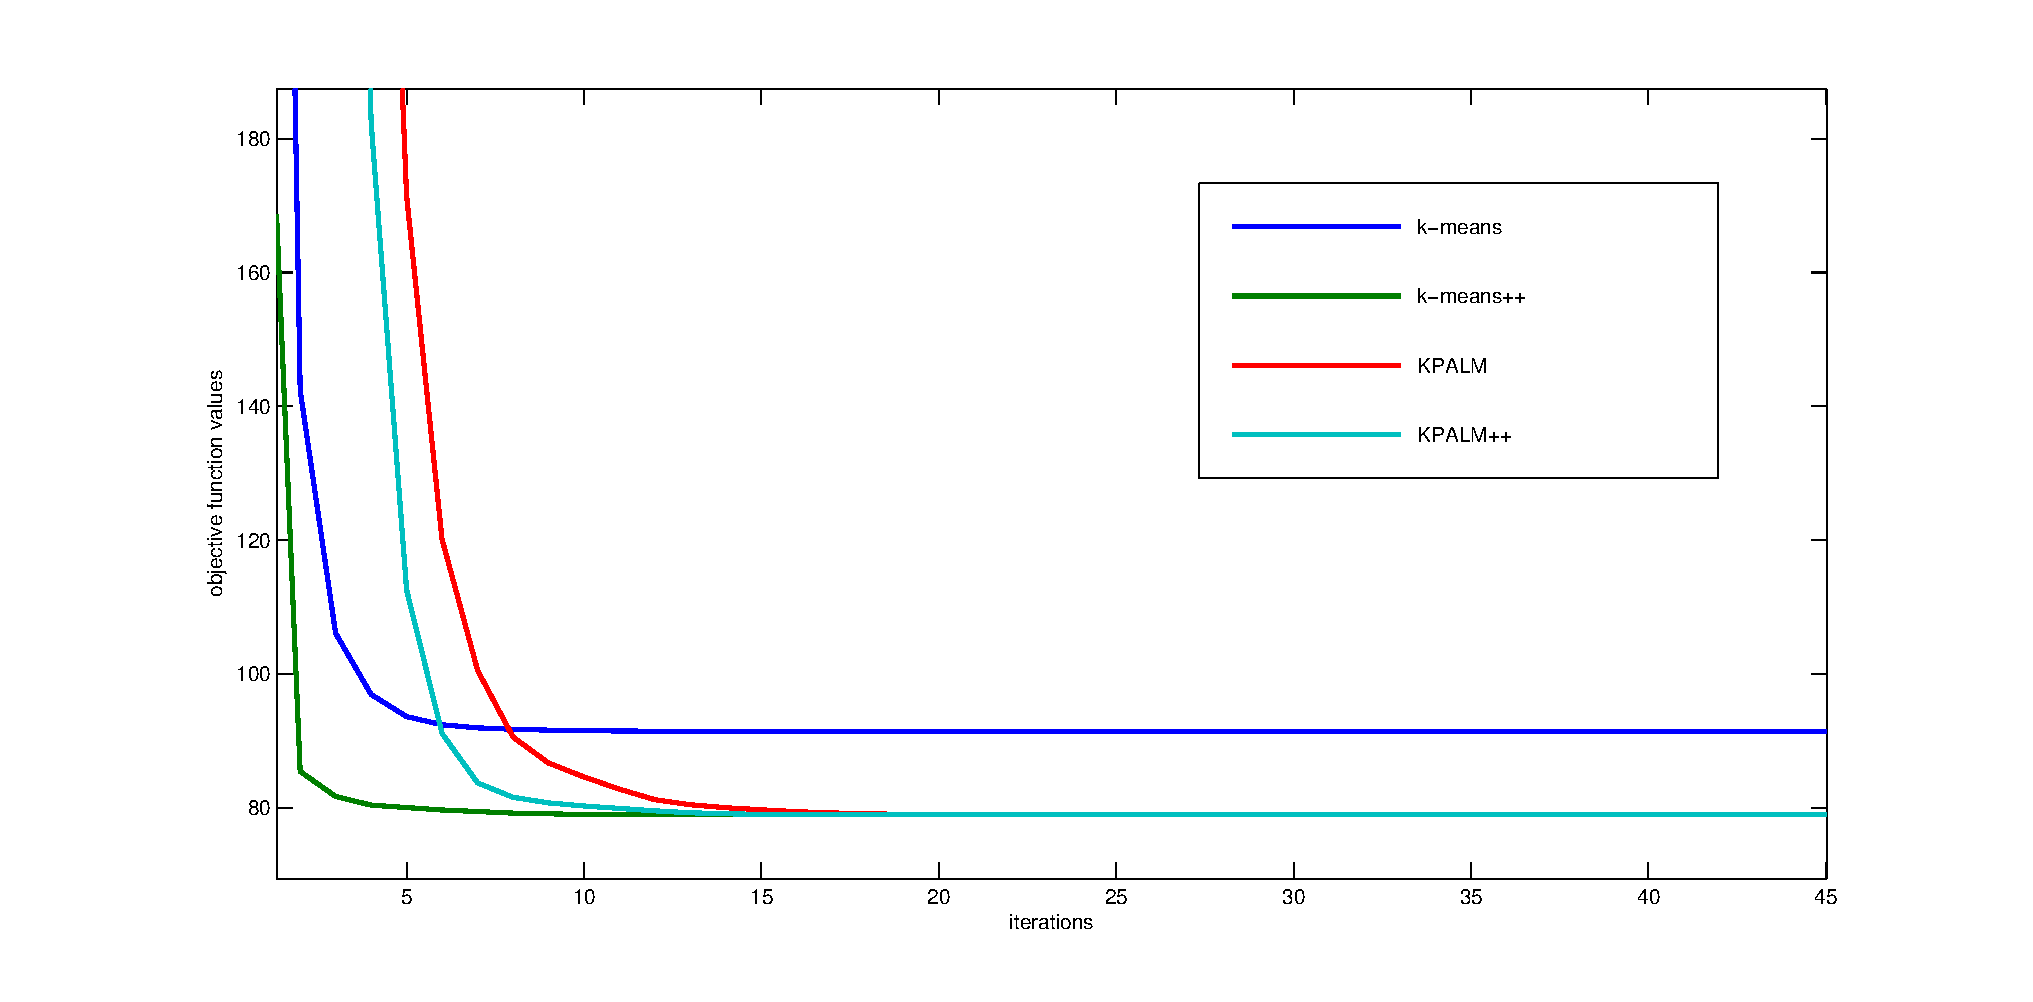
\includegraphics[width=0.75 \textwidth]{squared_norm_obj_comp}
		\end{figure}

	    	\item In the squared Euclidean setting, KPALM achieves lower objective function values than k-means. When using a more sophisticated initialization step, such as the one in k-means++, then k-means++ and KPALM++ achieve similar objective function values.
			\item k-means needs less number of iterations then KPALM to reach a certain precision.
		\end{itemize}
	\end{frame}	
	
	\begin{frame}{Numerical Results: The Squared Norm}
		\begin{itemize}[<+->]
            \item Comparison of the objective function values performed on the Iris dataset for KPALM algorithm with different $\alpha$ parameter updates.
		\begin{figure}
    		\centering
        	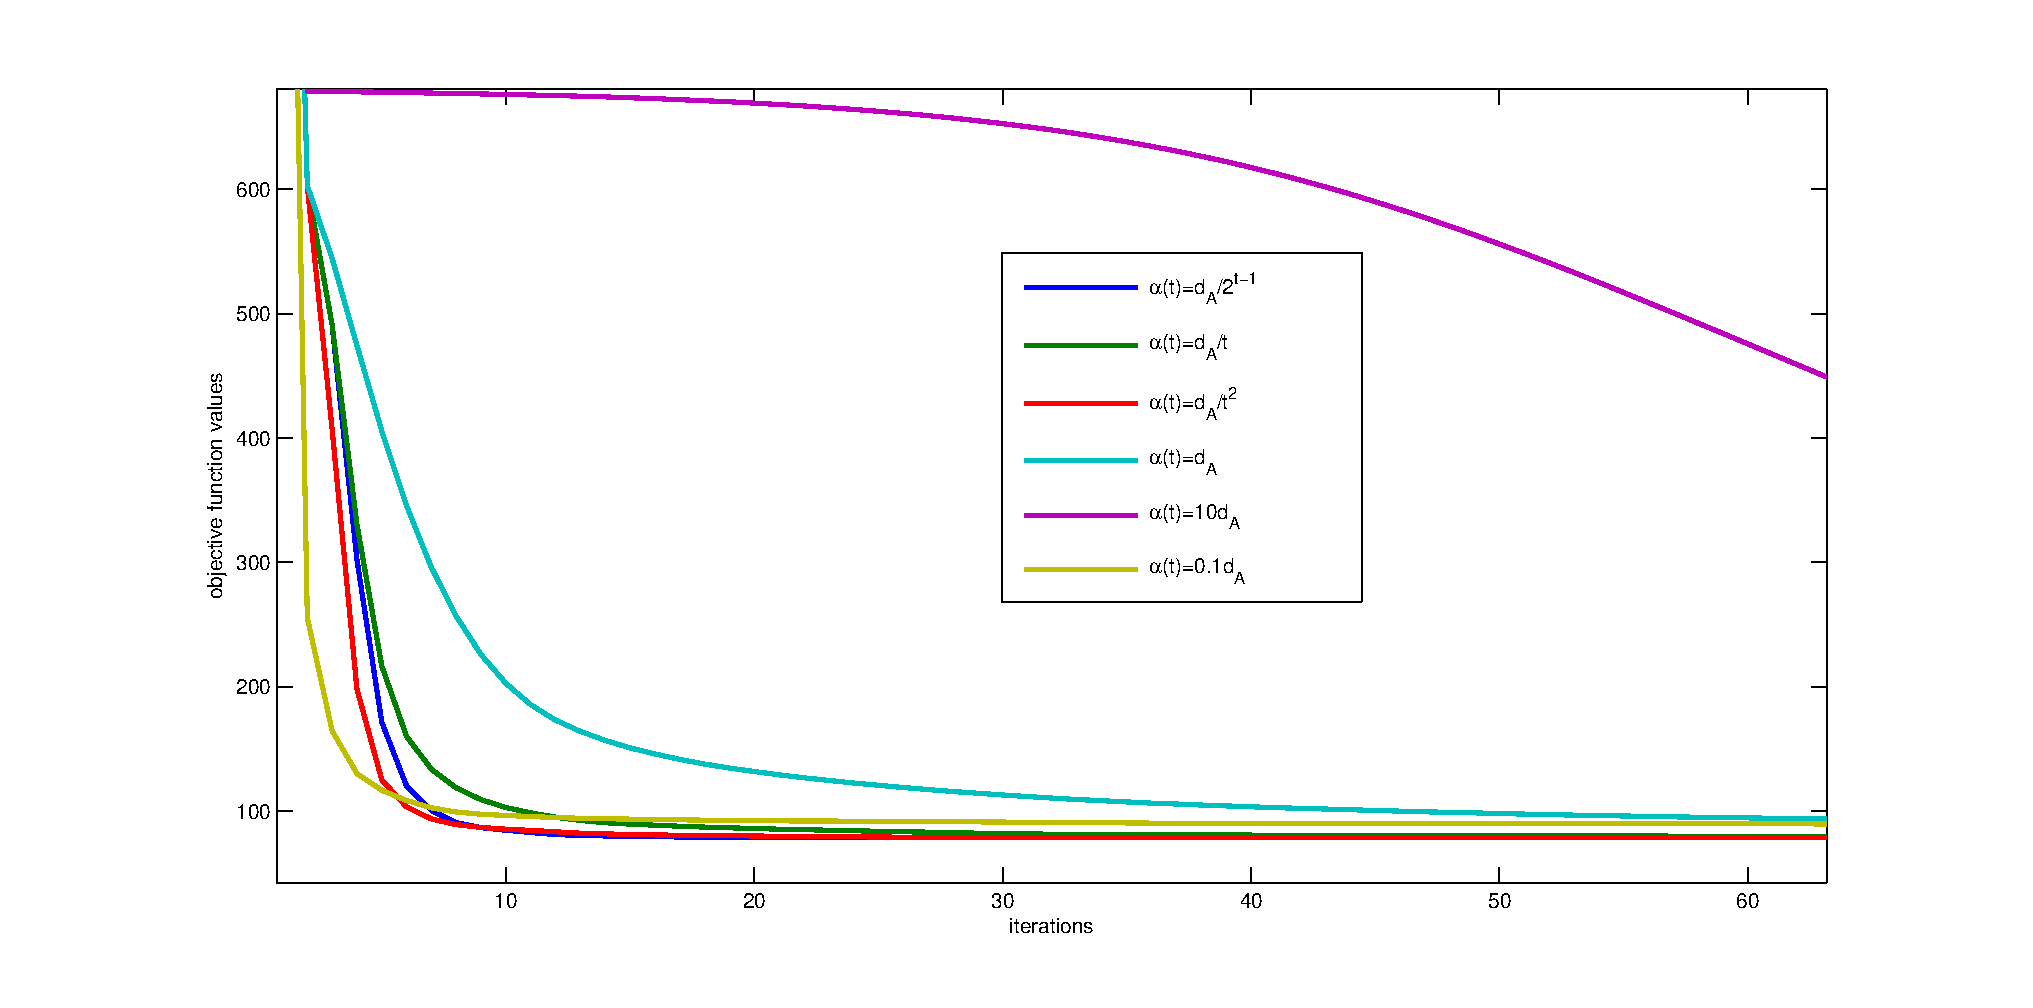
\includegraphics[width=0.8 \textwidth]{squared_norm_dyn_alpha_comp}
		\end{figure}
			\item It is preferable to use dynamic update of $\alpha(t)$ parameter to achieve a faster convergence, both in KPALM and $\epsilon$-KPALM. Example for suitable choices can be $\alpha(t)= \diam(\mathcal{A})/t$ and $\alpha(t)= \diam(\mathcal{A})/2^t$.
		\end{itemize}
	\end{frame}
	
	\begin{frame}{Numerical Results: Squared Norm Algorithms vs. $\varepsilon$-KPALM}
		\begin{itemize}[<+->]
			\item Generated two synthetic datasets, each 300 points
			\begin{figure}
		    	\centering
		    	\subfigure[Dense Gaussians]{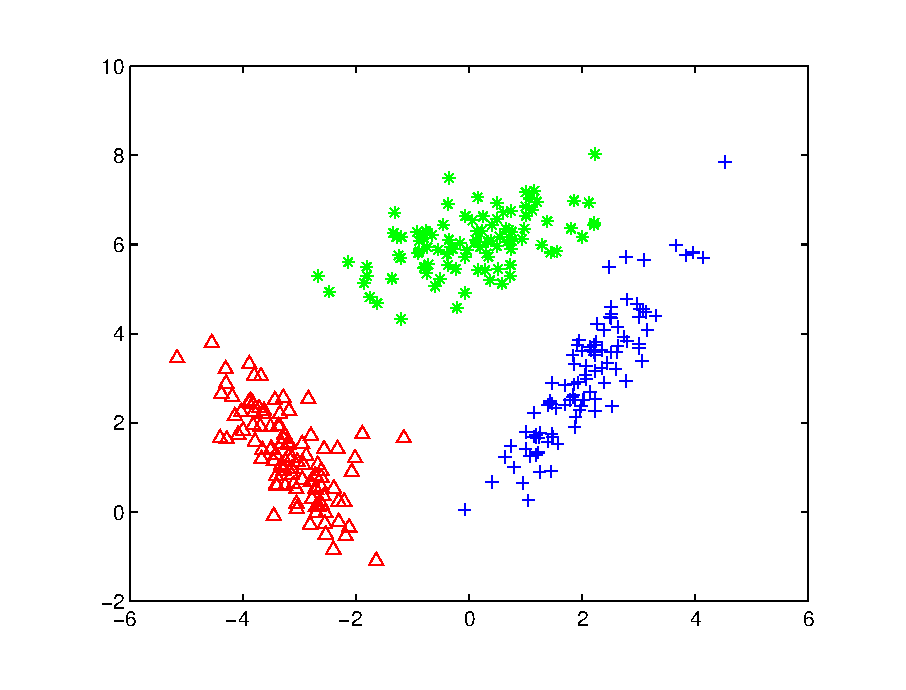
\includegraphics[width=0.45\textwidth]{dense_gaussians}}
				\subfigure[Sparse Gaussians]{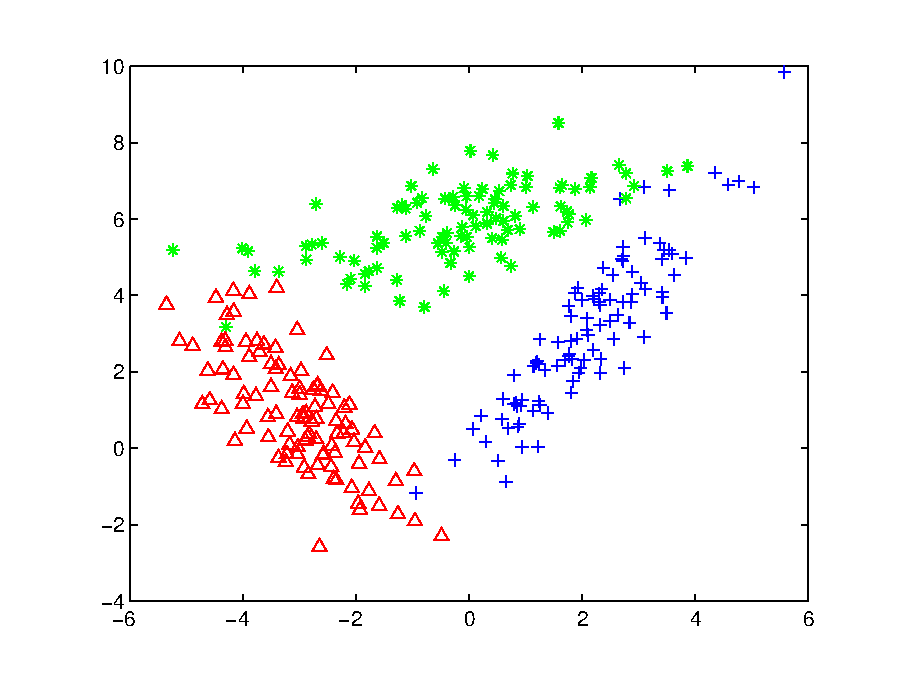
\includegraphics[width=0.45\textwidth]{sparse_gaussians}}
			\end{figure}
			\setcounter{subfigure}{0}
			\item Compared the resulting clustering using metrics, such as {\dblue Variation of Information} defined by:
				$VI(\mathcal{C}^1,\mathcal{C}^2):=-\sum\limits_{i,j} r_{i,j}\left[ \log \left( r_{i,j}/p_i \right) + \log \left( r_{i,j}/q_j \right) \right]$, where $\mathcal{C}^1=\left\lbrace C^1_1, C^1_2, \ldots C^1_k \right\rbrace$ and $\mathcal{C}^2=\left\lbrace C^2_1, C^2_2, \ldots C^2_l \right\rbrace$ are two clusterings of $\mathcal{A}$,\\ and $m=|\mathcal{A}|, \quad p_i=|C^1_i|/m,\quad q_j=|C^2_j|/m, \quad r_{i,j}= |C^1_i \cap C^2_j|/m$.
		\end{itemize}
	\end{frame}
	
	\begin{frame}{Numerical Results: Squared Norm Algorithms vs. $\varepsilon$-KPALM}
		\setcounter{subfigure}{0}
		\begin{figure}
		    \centering
		    \subfigure[Dense Gaussians metrics comparison]{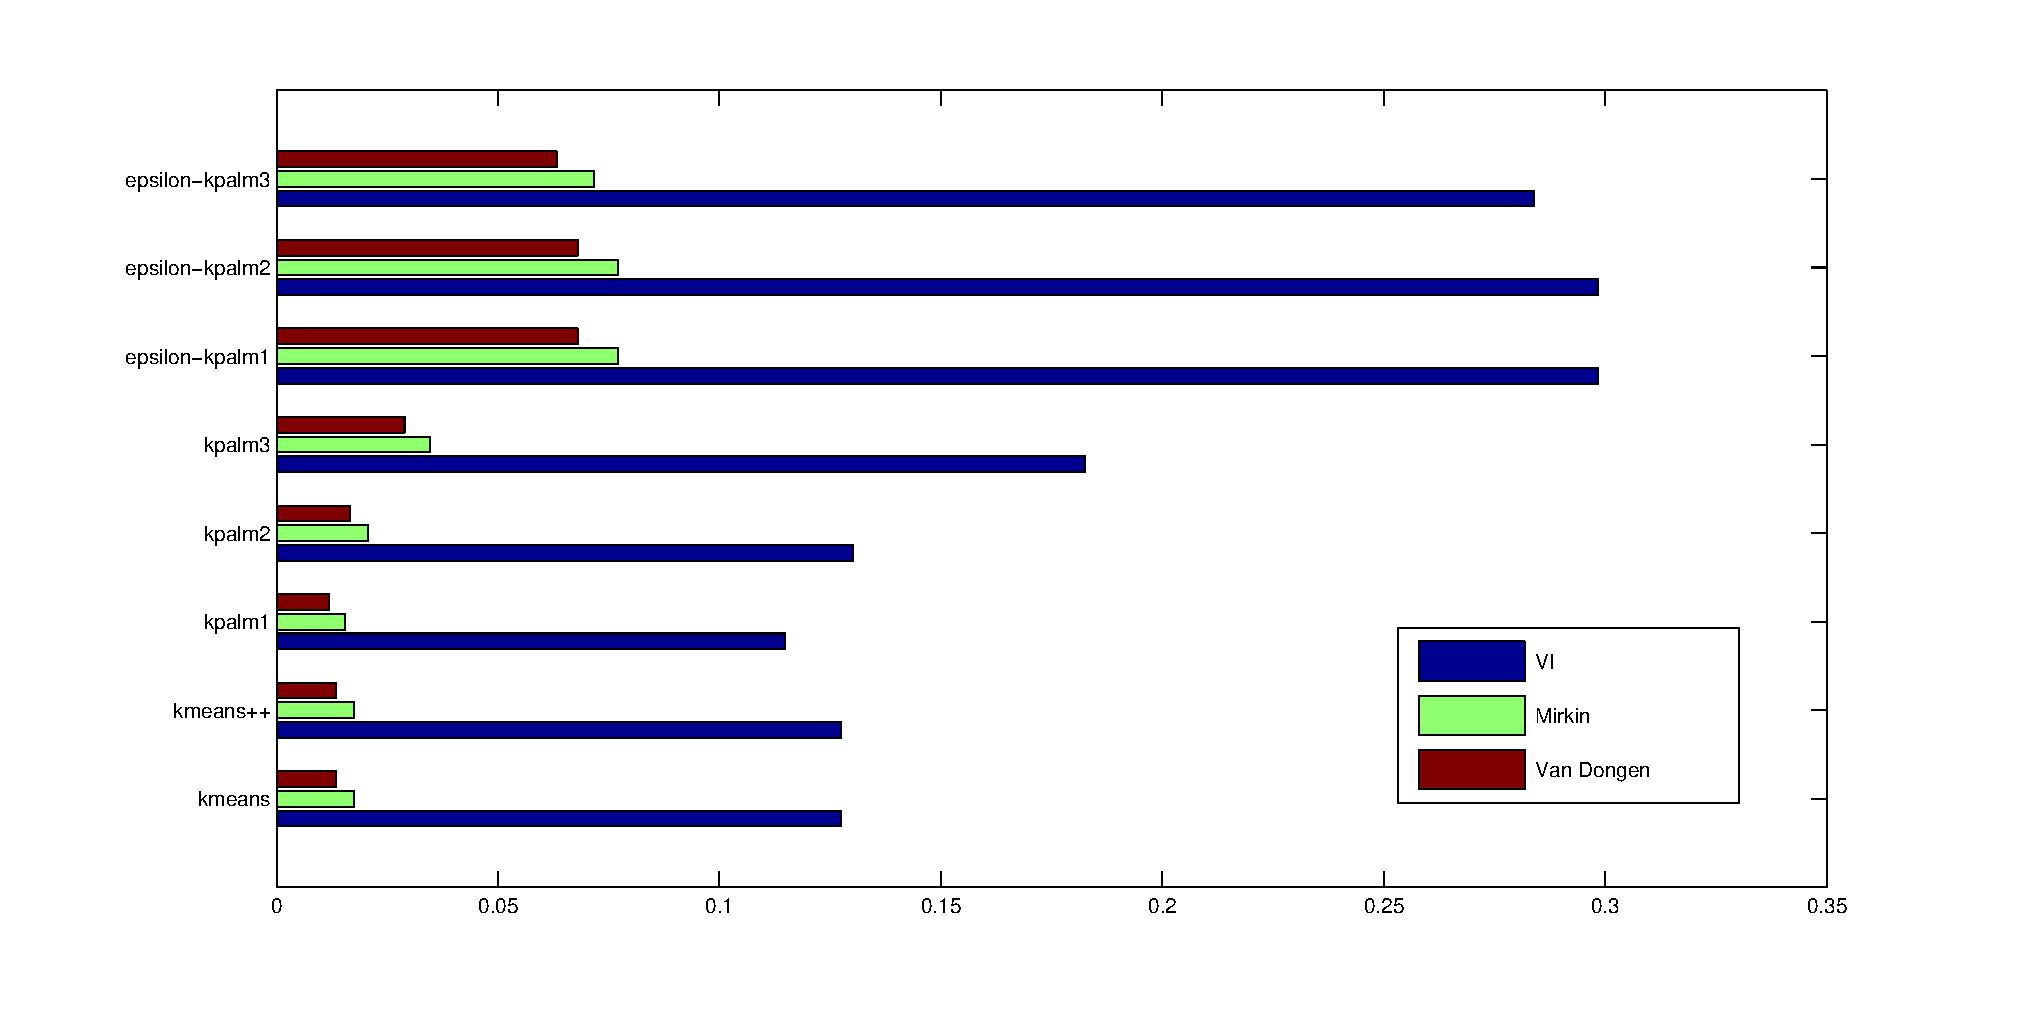
\includegraphics[width=0.45\textwidth]{dense_gaussians_metrics2}}
			\subfigure[Sparse Gaussians metrics comparison]{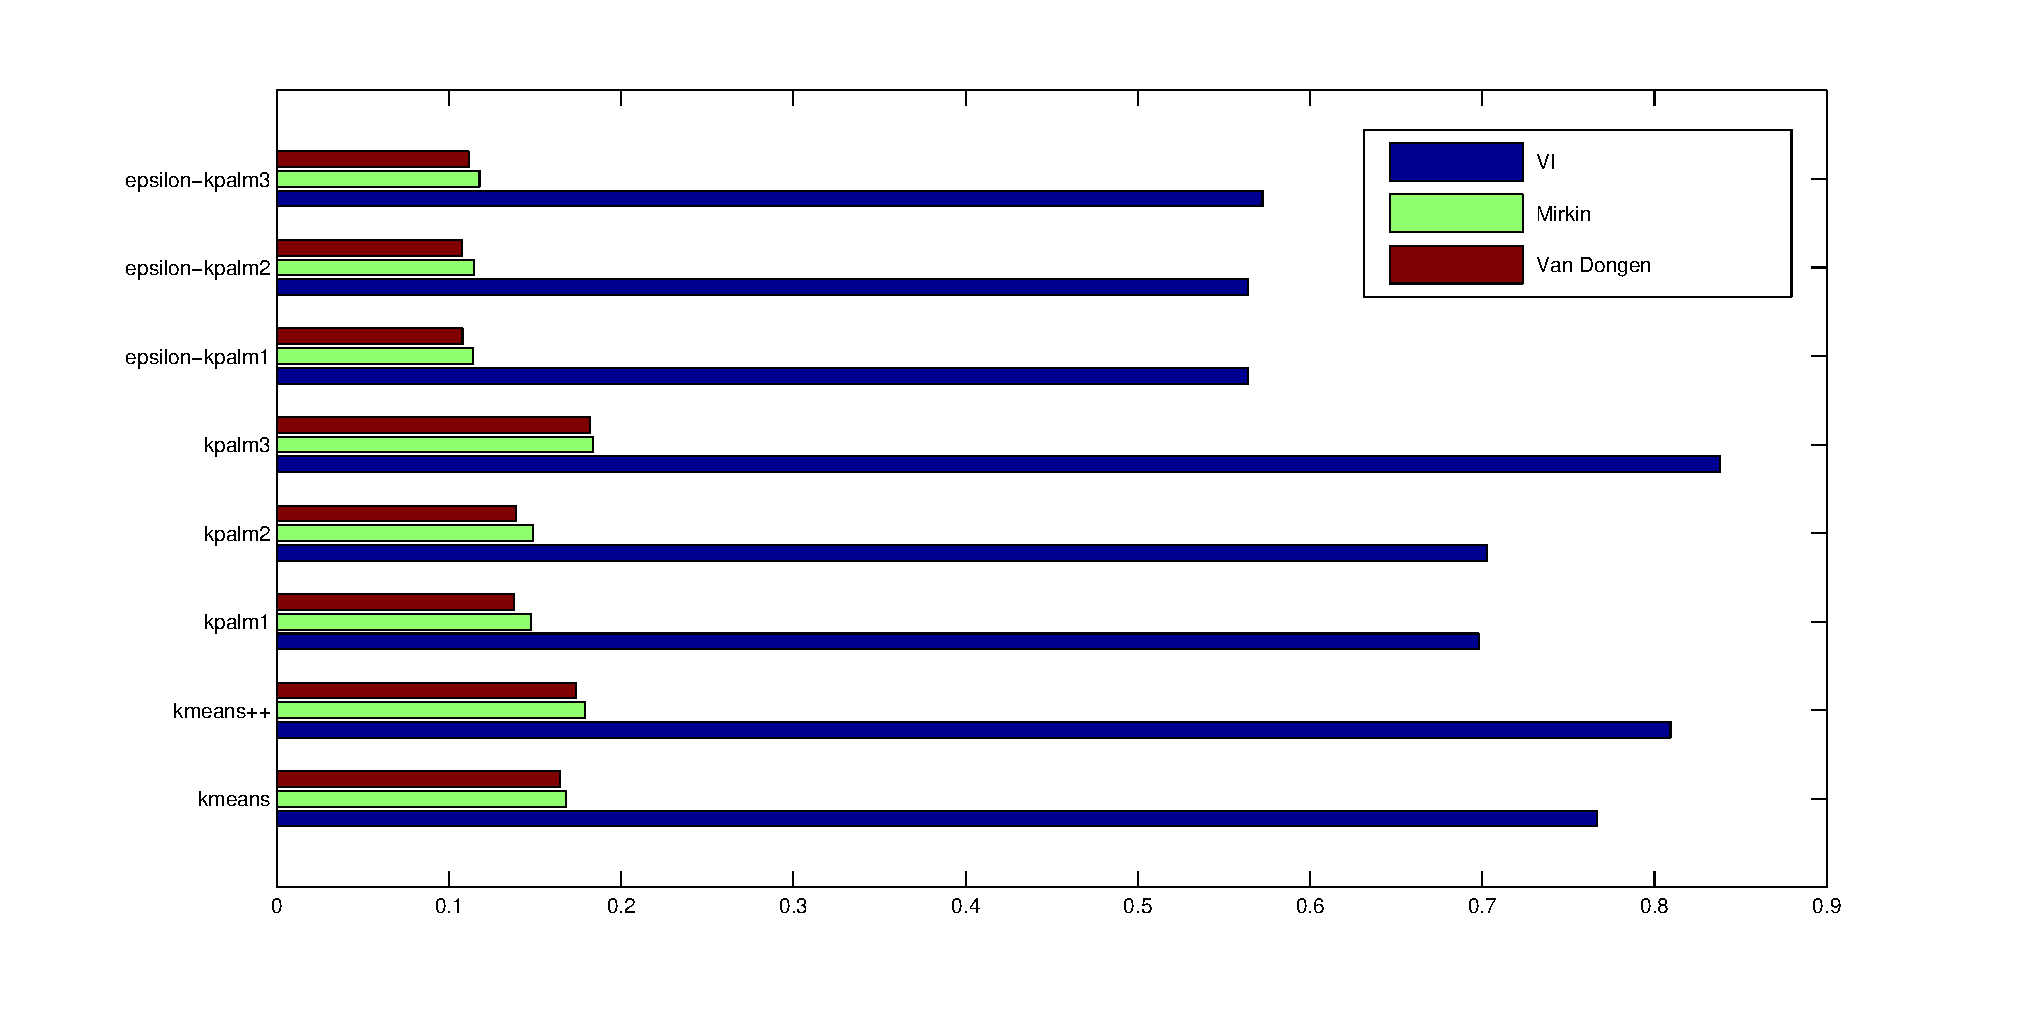
\includegraphics[width=0.45\textwidth]{sparse_gaussians_metrics2}}
		\end{figure}
		\pause
		\begin{itemize}[<+->]
			\item When the convex hulls of the desired clusters are mutually exclusive, algorithms which solve the clustering problem with the squared Euclidean distance are preferable to $\varepsilon$-KPALM.
			\item In datasets with outliers, the clustering obtained with $\varepsilon$-KPALM is more similar to the desired clustering, in terms of clustering metrics, than the clusterings obtained via the squared Euclidean algorithms. 
				Therefore, as expected, for data  with outliers, the choice of a norm instead of the squared norm is a more natural choice, and the $\varepsilon$-KPALM algorithm appears to be a promising algorithm to handle such data.
		\end{itemize}
	\end{frame}		
	
%	\begin{frame}{Summary of Numerical Results}
%		 \begin{itemize}[<+->]
%	    	\item In the squared Euclidean setting, KPALM achieves lower objective function values than k-means. When using a more sophisticated initialization step, such as the one in k-means++, then k-means++ and KPALM++ achieve similar objective function values.
%	\item k-means needs less number of iterations then KPALM to reach a certain precision.
%	\item It is preferable to use dynamic update of $\alpha(t)$ parameter to achieve a faster convergence, both in KPALM and $\epsilon$-KPALM. Example for suitable choices can be $\alpha(t)= \diam(\mathcal{A})/t$ and $\alpha(t)= \diam(\mathcal{A})/2^t$.
%	\item When the convex hulls of the desired clusters are mutually exclusive, algorithms which solve the clustering problem with the squared Euclidean distance are preferable to $\varepsilon$-KPALM.
%	\item In datasets with outliers, the clustering obtained with $\varepsilon$-KPALM is more similar to the desired clustering, in terms of clustering metrics, than the clusterings obtained via the squared Euclidean algorithms. 
%	Therefore, as expected, for data  with outliers, the choice of a norm instead of the squared norm is a more natural choice, and the $\varepsilon$-KPALM algorithm appears to be a promising algorithm to handle such data.	
%		\end{itemize}
%	\end{frame}
	
\end{document}

